%********************************************%
%*       Generated from PreTeXt source      *%
%*       on 2023-08-14T19:29:30Z       *%
%*   A recent stable commit (2022-07-01):   *%
%* 6c761d3dba23af92cba35001c852aac04ae99a5f *%
%*                                          *%
%*         https://pretextbook.org          *%
%*                                          *%
%********************************************%
\documentclass[oneside,10pt,]{book}
%% Custom Preamble Entries, early (use latex.preamble.early)
%% Default LaTeX packages
%%   1.  always employed (or nearly so) for some purpose, or
%%   2.  a stylewriter may assume their presence
\usepackage{geometry}
%% Some aspects of the preamble are conditional,
%% the LaTeX engine is one such determinant
\usepackage{ifthen}
%% etoolbox has a variety of modern conveniences
\usepackage{etoolbox}
\usepackage{ifxetex,ifluatex}
%% Raster graphics inclusion
\usepackage{graphicx}
%% Color support, xcolor package
%% Always loaded, for: add/delete text, author tools
%% Here, since tcolorbox loads tikz, and tikz loads xcolor
\PassOptionsToPackage{usenames,dvipsnames,svgnames,table}{xcolor}
\usepackage{xcolor}
%% begin: defined colors, via xcolor package, for styling
%% end: defined colors, via xcolor package, for styling
%% Colored boxes, and much more, though mostly styling
%% skins library provides "enhanced" skin, employing tikzpicture
%% boxes may be configured as "breakable" or "unbreakable"
%% "raster" controls grids of boxes, aka side-by-side
\usepackage{tcolorbox}
\tcbuselibrary{skins}
\tcbuselibrary{breakable}
\tcbuselibrary{raster}
%% We load some "stock" tcolorbox styles that we use a lot
%% Placement here is provisional, there will be some color work also
%% First, black on white, no border, transparent, but no assumption about titles
\tcbset{ bwminimalstyle/.style={size=minimal, boxrule=-0.3pt, frame empty,
colback=white, colbacktitle=white, coltitle=black, opacityfill=0.0} }
%% Second, bold title, run-in to text/paragraph/heading
%% Space afterwards will be controlled by environment,
%% independent of constructions of the tcb title
%% Places \blocktitlefont onto many block titles
\tcbset{ runintitlestyle/.style={fonttitle=\blocktitlefont\upshape\bfseries, attach title to upper} }
%% Spacing prior to each exercise, anywhere
\tcbset{ exercisespacingstyle/.style={before skip={1.5ex plus 0.5ex}} }
%% Spacing prior to each block
\tcbset{ blockspacingstyle/.style={before skip={2.0ex plus 0.5ex}} }
%% xparse allows the construction of more robust commands,
%% this is a necessity for isolating styling and behavior
%% The tcolorbox library of the same name loads the base library
\tcbuselibrary{xparse}
%% The tcolorbox library loads TikZ, its calc package is generally useful,
%% and is necessary for some smaller documents that use partial tcolor boxes
%% See:  https://github.com/PreTeXtBook/pretext/issues/1624
\usetikzlibrary{calc}
%% Hyperref should be here, but likes to be loaded late
%%
%% Inline math delimiters, \(, \), need to be robust
%% 2016-01-31:  latexrelease.sty  supersedes  fixltx2e.sty
%% If  latexrelease.sty  exists, bugfix is in kernel
%% If not, bugfix is in  fixltx2e.sty
%% See:  https://tug.org/TUGboat/tb36-3/tb114ltnews22.pdf
%% and read "Fewer fragile commands" in distribution's  latexchanges.pdf
\IfFileExists{latexrelease.sty}{}{\usepackage{fixltx2e}}
%% Text height identically 9 inches, text width varies on point size
%% See Bringhurst 2.1.1 on measure for recommendations
%% 75 characters per line (count spaces, punctuation) is target
%% which is the upper limit of Bringhurst's recommendations
\geometry{letterpaper,total={340pt,9.0in}}
%% Custom Page Layout Adjustments (use publisher page-geometry entry)
%% This LaTeX file may be compiled with pdflatex, xelatex, or lualatex executables
%% LuaTeX is not explicitly supported, but we do accept additions from knowledgeable users
%% The conditional below provides  pdflatex  specific configuration last
%% begin: engine-specific capabilities
\ifthenelse{\boolean{xetex} \or \boolean{luatex}}{%
%% begin: xelatex and lualatex-specific default configuration
\ifxetex\usepackage{xltxtra}\fi
%% realscripts is the only part of xltxtra relevant to lualatex 
\ifluatex\usepackage{realscripts}\fi
%% end:   xelatex and lualatex-specific default configuration
}{
%% begin: pdflatex-specific default configuration
%% We assume a PreTeXt XML source file may have Unicode characters
%% and so we ask LaTeX to parse a UTF-8 encoded file
%% This may work well for accented characters in Western language,
%% but not with Greek, Asian languages, etc.
%% When this is not good enough, switch to the  xelatex  engine
%% where Unicode is better supported (encouraged, even)
\usepackage[utf8]{inputenc}
%% end: pdflatex-specific default configuration
}
%% end:   engine-specific capabilities
%%
%% Fonts.  Conditional on LaTex engine employed.
%% Default Text Font: The Latin Modern fonts are
%% "enhanced versions of the [original TeX] Computer Modern fonts."
%% We use them as the default text font for PreTeXt output.
%% Automatic Font Control
%% Portions of a document, are, or may, be affected by defined commands
%% These are perhaps more flexible when using  xelatex  rather than  pdflatex
%% The following definitions are meant to be re-defined in a style, using \renewcommand
%% They are scoped when employed (in a TeX group), and so should not be defined with an argument
\newcommand{\divisionfont}{\relax}
\newcommand{\blocktitlefont}{\relax}
\newcommand{\contentsfont}{\relax}
\newcommand{\pagefont}{\relax}
\newcommand{\tabularfont}{\relax}
\newcommand{\xreffont}{\relax}
\newcommand{\titlepagefont}{\relax}
%%
\ifthenelse{\boolean{xetex} \or \boolean{luatex}}{%
%% begin: font setup and configuration for use with xelatex
%% Generally, xelatex is necessary for non-Western fonts
%% fontspec package provides extensive control of system fonts,
%% meaning *.otf (OpenType), and apparently *.ttf (TrueType)
%% that live *outside* your TeX/MF tree, and are controlled by your *system*
%% (it is possible that a TeX distribution will place fonts in a system location)
%%
%% The fontspec package is the best vehicle for using different fonts in  xelatex
%% So we load it always, no matter what a publisher or style might want
%%
\usepackage{fontspec}
%%
%% begin: xelatex main font ("font-xelatex-main" template)
%% Latin Modern Roman is the default font for xelatex and so is loaded with a TU encoding
%% *in the format* so we can't touch it, only perhaps adjust it later
%% in one of two ways (then known by NFSS names such as "lmr")
%% (1) via NFSS with font family names such as "lmr" and "lmss"
%% (2) via fontspec with commands like \setmainfont{Latin Modern Roman}
%% The latter requires the font to be known at the system-level by its font name,
%% but will give access to OTF font features through optional arguments
%% https://tex.stackexchange.com/questions/470008/
%% where-and-how-does-fontspec-sty-specify-the-default-font-latin-modern-roman
%% http://tex.stackexchange.com/questions/115321
%% /how-to-optimize-latin-modern-font-with-xelatex
%%
%% end:   xelatex main font ("font-xelatex-main" template)
%% begin: xelatex mono font ("font-xelatex-mono" template)
%% (conditional on non-trivial uses being present in source)
%% end:   xelatex mono font ("font-xelatex-mono" template)
%% begin: xelatex font adjustments ("font-xelatex-style" template)
%% end:   xelatex font adjustments ("font-xelatex-style" template)
%%
%% Extensive support for other languages
\usepackage{polyglossia}
%% Set main/default language based on pretext/@xml:lang value
%% document language code is "en-US", US English
%% usmax variant has extra hypenation
\setmainlanguage[variant=usmax]{english}
%% Enable secondary languages based on discovery of @xml:lang values
%% Enable fonts/scripts based on discovery of @xml:lang values
%% Western languages should be ably covered by Latin Modern Roman
%% end:   font setup and configuration for use with xelatex
}{%
%% begin: font setup and configuration for use with pdflatex
%% begin: pdflatex main font ("font-pdflatex-main" template)
\usepackage{lmodern}
\usepackage[T1]{fontenc}
%% end:   pdflatex main font ("font-pdflatex-main" template)
%% begin: pdflatex mono font ("font-pdflatex-mono" template)
%% (conditional on non-trivial uses being present in source)
%% end:   pdflatex mono font ("font-pdflatex-mono" template)
%% begin: pdflatex font adjustments ("font-pdflatex-style" template)
%% end:   pdflatex font adjustments ("font-pdflatex-style" template)
%% end:   font setup and configuration for use with pdflatex
}
%% Micromanage spacing, etc.  The named "microtype-options"
%% template may be employed to fine-tune package behavior
\usepackage{microtype}
%% Symbols, align environment, commutative diagrams, bracket-matrix
\usepackage{amsmath}
\usepackage{amscd}
\usepackage{amssymb}
%% allow page breaks within display mathematics anywhere
%% level 4 is maximally permissive
%% this is exactly the opposite of AMSmath package philosophy
%% there are per-display, and per-equation options to control this
%% split, aligned, gathered, and alignedat are not affected
\allowdisplaybreaks[4]
%% allow more columns to a matrix
%% can make this even bigger by overriding with  latex.preamble.late  processing option
\setcounter{MaxMatrixCols}{30}
%%
%%
%% Division Titles, and Page Headers/Footers
%% titlesec package, loading "titleps" package cooperatively
%% See code comments about the necessity and purpose of "explicit" option.
%% The "newparttoc" option causes a consistent entry for parts in the ToC 
%% file, but it is only effective if there is a \titleformat for \part.
%% "pagestyles" loads the  titleps  package cooperatively.
\usepackage[explicit, newparttoc, pagestyles]{titlesec}
%% The companion titletoc package for the ToC.
\usepackage{titletoc}
%% Fixes a bug with transition from chapters to appendices in a "book"
%% See generating XSL code for more details about necessity
\newtitlemark{\chaptertitlename}
%% begin: customizations of page styles via the modal "titleps-style" template
%% Designed to use commands from the LaTeX "titleps" package
%% Plain pages should have the same font for page numbers
\renewpagestyle{plain}{%
\setfoot{}{\pagefont\thepage}{}%
}%
%% Single pages as in default LaTeX
\renewpagestyle{headings}{%
\sethead{\pagefont\slshape\MakeUppercase{\ifthechapter{\chaptertitlename\space\thechapter.\space}{}\chaptertitle}}{}{\pagefont\thepage}%
}%
\pagestyle{headings}
%% end: customizations of page styles via the modal "titleps-style" template
%%
%% Create globally-available macros to be provided for style writers
%% These are redefined for each occurence of each division
\newcommand{\divisionnameptx}{\relax}%
\newcommand{\titleptx}{\relax}%
\newcommand{\subtitleptx}{\relax}%
\newcommand{\shortitleptx}{\relax}%
\newcommand{\authorsptx}{\relax}%
\newcommand{\epigraphptx}{\relax}%
%% Create environments for possible occurences of each division
%% Environment for a PTX "acknowledgement" at the level of a LaTeX "chapter"
\NewDocumentEnvironment{acknowledgement}{mmmmmmm}
{%
\renewcommand{\divisionnameptx}{#1}%
\renewcommand{\titleptx}{#2}%
\renewcommand{\subtitleptx}{#3}%
\renewcommand{\shortitleptx}{#4}%
\renewcommand{\authorsptx}{#5}%
\renewcommand{\epigraphptx}{#6}%
\chapter*{#2}%
\addcontentsline{toc}{chapter}{#4}
\label{#7}%
}{}%
%% Environment for a PTX "preface" at the level of a LaTeX "chapter"
\NewDocumentEnvironment{preface}{mmmmmmm}
{%
\renewcommand{\divisionnameptx}{#1}%
\renewcommand{\titleptx}{#2}%
\renewcommand{\subtitleptx}{#3}%
\renewcommand{\shortitleptx}{#4}%
\renewcommand{\authorsptx}{#5}%
\renewcommand{\epigraphptx}{#6}%
\chapter*{#2}%
\addcontentsline{toc}{chapter}{#4}
\label{#7}%
}{}%
%% Environment for a PTX "chapter" at the level of a LaTeX "chapter"
\NewDocumentEnvironment{chapterptx}{mmmmmmm}
{%
\renewcommand{\divisionnameptx}{#1}%
\renewcommand{\titleptx}{#2}%
\renewcommand{\subtitleptx}{#3}%
\renewcommand{\shortitleptx}{#4}%
\renewcommand{\authorsptx}{#5}%
\renewcommand{\epigraphptx}{#6}%
\chapter[{#4}]{#2}%
\label{#7}%
}{}%
%% Environment for a PTX "section" at the level of a LaTeX "section"
\NewDocumentEnvironment{sectionptx}{mmmmmmm}
{%
\renewcommand{\divisionnameptx}{#1}%
\renewcommand{\titleptx}{#2}%
\renewcommand{\subtitleptx}{#3}%
\renewcommand{\shortitleptx}{#4}%
\renewcommand{\authorsptx}{#5}%
\renewcommand{\epigraphptx}{#6}%
\section[{#4}]{#2}%
\label{#7}%
}{}%
%% Environment for a PTX "subsection" at the level of a LaTeX "subsection"
\NewDocumentEnvironment{subsectionptx}{mmmmmmm}
{%
\renewcommand{\divisionnameptx}{#1}%
\renewcommand{\titleptx}{#2}%
\renewcommand{\subtitleptx}{#3}%
\renewcommand{\shortitleptx}{#4}%
\renewcommand{\authorsptx}{#5}%
\renewcommand{\epigraphptx}{#6}%
\subsection[{#4}]{#2}%
\label{#7}%
}{}%
%% Environment for a PTX "exercises" at the level of a LaTeX "subsection"
\NewDocumentEnvironment{exercises-subsection}{mmmmmmm}
{%
\renewcommand{\divisionnameptx}{#1}%
\renewcommand{\titleptx}{#2}%
\renewcommand{\subtitleptx}{#3}%
\renewcommand{\shortitleptx}{#4}%
\renewcommand{\authorsptx}{#5}%
\renewcommand{\epigraphptx}{#6}%
\subsection[{#4}]{#2}%
\label{#7}%
}{}%
%% Environment for a PTX "exercises" at the level of a LaTeX "subsection"
\NewDocumentEnvironment{exercises-subsection-numberless}{mmmmmmm}
{%
\renewcommand{\divisionnameptx}{#1}%
\renewcommand{\titleptx}{#2}%
\renewcommand{\subtitleptx}{#3}%
\renewcommand{\shortitleptx}{#4}%
\renewcommand{\authorsptx}{#5}%
\renewcommand{\epigraphptx}{#6}%
\subsection*{#2}%
\addcontentsline{toc}{subsection}{#4}
\label{#7}%
}{}%
%% Environment for a PTX "index" at the level of a LaTeX "chapter"
\NewDocumentEnvironment{indexptx}{mmmmmmm}
{%
\renewcommand{\divisionnameptx}{#1}%
\renewcommand{\titleptx}{#2}%
\renewcommand{\subtitleptx}{#3}%
\renewcommand{\shortitleptx}{#4}%
\renewcommand{\authorsptx}{#5}%
\renewcommand{\epigraphptx}{#6}%
\chapter*{#2}%
\addcontentsline{toc}{chapter}{#4}
\label{#7}%
}{}%
%%
%% Styles for six traditional LaTeX divisions
\titleformat{\part}[display]
{\divisionfont\Huge\bfseries\centering}{\divisionnameptx\space\thepart}{30pt}{\Huge#1}
[{\Large\centering\authorsptx}]
\titleformat{\chapter}[display]
{\divisionfont\huge\bfseries}{\divisionnameptx\space\thechapter}{20pt}{\Huge#1}
[{\Large\authorsptx}]
\titleformat{name=\chapter,numberless}[display]
{\divisionfont\huge\bfseries}{}{0pt}{#1}
[{\Large\authorsptx}]
\titlespacing*{\chapter}{0pt}{50pt}{40pt}
\titleformat{\section}[hang]
{\divisionfont\Large\bfseries}{\thesection}{1ex}{#1}
[{\large\authorsptx}]
\titleformat{name=\section,numberless}[block]
{\divisionfont\Large\bfseries}{}{0pt}{#1}
[{\large\authorsptx}]
\titlespacing*{\section}{0pt}{3.5ex plus 1ex minus .2ex}{2.3ex plus .2ex}
\titleformat{\subsection}[hang]
{\divisionfont\large\bfseries}{\thesubsection}{1ex}{#1}
[{\normalsize\authorsptx}]
\titleformat{name=\subsection,numberless}[block]
{\divisionfont\large\bfseries}{}{0pt}{#1}
[{\normalsize\authorsptx}]
\titlespacing*{\subsection}{0pt}{3.25ex plus 1ex minus .2ex}{1.5ex plus .2ex}
\titleformat{\subsubsection}[hang]
{\divisionfont\normalsize\bfseries}{\thesubsubsection}{1em}{#1}
[{\small\authorsptx}]
\titleformat{name=\subsubsection,numberless}[block]
{\divisionfont\normalsize\bfseries}{}{0pt}{#1}
[{\normalsize\authorsptx}]
\titlespacing*{\subsubsection}{0pt}{3.25ex plus 1ex minus .2ex}{1.5ex plus .2ex}
\titleformat{\paragraph}[hang]
{\divisionfont\normalsize\bfseries}{\theparagraph}{1em}{#1}
[{\small\authorsptx}]
\titleformat{name=\paragraph,numberless}[block]
{\divisionfont\normalsize\bfseries}{}{0pt}{#1}
[{\normalsize\authorsptx}]
\titlespacing*{\paragraph}{0pt}{3.25ex plus 1ex minus .2ex}{1.5em}
%%
%% Styles for five traditional LaTeX divisions
\titlecontents{part}%
[0pt]{\contentsmargin{0em}\addvspace{1pc}\contentsfont\bfseries}%
{\Large\thecontentslabel\enspace}{\Large}%
{}%
[\addvspace{.5pc}]%
\titlecontents{chapter}%
[0pt]{\contentsmargin{0em}\addvspace{1pc}\contentsfont\bfseries}%
{\large\thecontentslabel\enspace}{\large}%
{\hfill\bfseries\thecontentspage}%
[\addvspace{.5pc}]%
\dottedcontents{section}[3.8em]{\contentsfont}{2.3em}{1pc}%
\dottedcontents{subsection}[6.1em]{\contentsfont}{3.2em}{1pc}%
\dottedcontents{subsubsection}[9.3em]{\contentsfont}{4.3em}{1pc}%
%%
%% Begin: Semantic Macros
%% To preserve meaning in a LaTeX file
%%
%% \mono macro for content of "c", "cd", "tag", etc elements
%% Also used automatically in other constructions
%% Simply an alias for \texttt
%% Always defined, even if there is no need, or if a specific tt font is not loaded
\newcommand{\mono}[1]{\texttt{#1}}
%%
%% Following semantic macros are only defined here if their
%% use is required only in this specific document
%%
%% Used for inline definitions of terms
\newcommand{\terminology}[1]{\textbf{#1}}
%% Used for fillin answer blank in text
%% Relies on calc package, loaded via tcolorbox
%% Argument is intended number of characters of blank
%% Length may compress for output to fit in one line
\newlength{\fillinmaxwidth}
\newlength{\fillincontract}
\newlength{\fillinheight}
\newcommand{\fillintext}[1]{%
\setlength{\fillinmaxwidth}{#1em*\real{0.5}}%
\setlength{\fillincontract}{#1em*\real{0.5}*\real{0.2}}%
\setlength{\fillinheight}{\heightof{\strut}+1.2pt}%
\strut\nobreak\leaders\vbox{\hrule width 0.3pt height 0.3pt \vskip -1.2pt}\hskip 1\fillinmaxwidth minus \fillincontract\nobreak\strut%
}
%% End: Semantic Macros
%% Divisional exercises (and worksheet) as LaTeX environments
%% Third argument is option for extra workspace in worksheets
%% Hanging indent occupies a 5ex width slot prior to left margin
%% Experimentally this seems just barely sufficient for a bold "888."
%% Division exercises, not in exercise group
\tcbset{ divisionexercisestyle/.style={bwminimalstyle, runintitlestyle, exercisespacingstyle, left=5ex, breakable, parbox=false } }
\newtcolorbox{divisionexercise}[4]{divisionexercisestyle, before title={\hspace{-5ex}\makebox[5ex][l]{#1.}}, title={\notblank{#2}{#2\space}{}}, phantom={\hypertarget{#4}{}}, after={\notblank{#3}{\newline\rule{\workspacestrutwidth}{#3}\newline\vfill}{\par}}}
%% "tcolorbox" environment for a single image, occupying entire \linewidth
%% arguments are left-margin, width, right-margin, as multiples of
%% \linewidth, and are guaranteed to be positive and sum to 1.0
\tcbset{ imagestyle/.style={bwminimalstyle} }
\NewTColorBox{tcbimage}{mmm}{imagestyle,left skip=#1\linewidth,width=#2\linewidth}
%% Wrapper environment for tcbimage environment with a fourth argument
%% Fourth argument, if nonempty, is a vertical space adjustment
%% and implies image will be preceded by \leavevmode\nopagebreak
%% Intended use is for alignment with a list marker
\NewDocumentEnvironment{image}{mmmm}{\notblank{#4}{\leavevmode\nopagebreak\vspace{#4}}{}\begin{tcbimage}{#1}{#2}{#3}}{\end{tcbimage}%
}%% More flexible list management, esp. for references
%% But also for specifying labels (i.e. custom order) on nested lists
\usepackage{enumitem}
%% Support for index creation
%% imakeidx package does not require extra pass (as with makeidx)
%% Title of the "Index" section set via a keyword
%% Language support for the "see" and "see also" phrases,
%% but to do so presumes exactly one "index-list" generator is present
\usepackage{imakeidx}
\makeindex[title=Index, intoc=true]
\renewcommand{\seename}{See}
\renewcommand{\alsoname}{See also}
%% hyperref driver does not need to be specified, it will be detected
%% Footnote marks in tcolorbox have broken linking under
%% hyperref, so it is necessary to turn off all linking
%% It *must* be given as a package option, not with \hypersetup
\usepackage[hyperfootnotes=false]{hyperref}
%% Hyperlinking active in electronic PDFs, all links without surrounding boxes and blue
\hypersetup{colorlinks=true,linkcolor=blue,citecolor=blue,filecolor=blue,urlcolor=blue}
%% Less-clever names for hyperlinks are more reliable, *especially* for structural parts
%% See comments in the code to learn more about the importance of this setting
\hypersetup{hypertexnames=false}
%%The  hypertexnames  setting then confuses the hyperlinking from the index
%%This patch resolves the incorrect links, see code for StackExchange post.
\makeatletter
\patchcmd\Hy@EveryPageBoxHook{\Hy@EveryPageAnchor}{\Hy@hypertexnamestrue\Hy@EveryPageAnchor}{}{\fail}
\makeatother
\hypersetup{pdftitle={Precalculus Review Materials}}
%% If you manually remove hyperref, leave in this next command
%% This will allow LaTeX compilation, employing this no-op command
\providecommand\phantomsection{}
%% Division Numbering: Chapters, Sections, Subsections, etc
%% Division numbers may be turned off at some level ("depth")
%% A section *always* has depth 1, contrary to us counting from the document root
%% The latex default is 3.  If a larger number is present here, then
%% removing this command may make some cross-references ambiguous
%% The precursor variable $numbering-maxlevel is checked for consistency in the common XSL file
\setcounter{secnumdepth}{3}
%%
%% AMS "proof" environment is no longer used, but we leave previously
%% implemented \qedhere in place, should the LaTeX be recycled
\newcommand{\qedhere}{\relax}
%%
%% A faux tcolorbox whose only purpose is to provide common numbering
%% facilities for most blocks (possibly not projects, 2D displays)
%% Controlled by  numbering.theorems.level  processing parameter
\newtcolorbox[auto counter, number within=section]{block}{}
%%
%% This document is set to number PROJECT-LIKE on a separate numbering scheme
%% So, a faux tcolorbox whose only purpose is to provide this numbering
%% Controlled by  numbering.projects.level  processing parameter
\newtcolorbox[auto counter, number within=section]{project-distinct}{}
%% A faux tcolorbox whose only purpose is to provide common numbering
%% facilities for 2D displays which are subnumbered as part of a "sidebyside"
\makeatletter
\newtcolorbox[auto counter, number within=tcb@cnt@block, number freestyle={\noexpand\thetcb@cnt@block(\noexpand\alph{\tcbcounter})}]{subdisplay}{}
\makeatother
%%
%% tcolorbox, with styles, for REMARK-LIKE
%%
%% warning: fairly simple numbered block/structure
\tcbset{ warningstyle/.style={bwminimalstyle, runintitlestyle, blockspacingstyle, after title={\space}, } }
\newtcolorbox[use counter from=block]{warning}[3]{title={{#1~\thetcbcounter\notblank{#2}{\space\space#2}{}}}, phantomlabel={#3}, breakable, parbox=false, after={\par}, warningstyle, }
%%
%% tcolorbox, with styles, for EXAMPLE-LIKE
%%
%% example: fairly simple numbered block/structure
\tcbset{ examplestyle/.style={bwminimalstyle, runintitlestyle, blockspacingstyle, after title={\space}, after upper={\space\space\hspace*{\stretch{1}}\(\square\)}, } }
\newtcolorbox[use counter from=block]{example}[3]{title={{#1~\thetcbcounter\notblank{#2}{\space\space#2}{}}}, phantomlabel={#3}, breakable, parbox=false, after={\par}, examplestyle, }
%%
%% tcolorbox, with styles, for inline exercises
%%
%% inlineexercise: fairly simple numbered block/structure
\tcbset{ inlineexercisestyle/.style={bwminimalstyle, runintitlestyle, blockspacingstyle, after title={\space}, } }
\newtcolorbox[use counter from=block]{inlineexercise}[3]{title={{#1~\thetcbcounter\notblank{#2}{\space\space#2}{}}}, phantomlabel={#3}, breakable, parbox=false, after={\par}, inlineexercisestyle, }
%%
%% tcolorbox, with styles, for FIGURE-LIKE
%%
%% figureptx: 2-D display structure
\tcbset{ figureptxstyle/.style={bwminimalstyle, middle=1ex, blockspacingstyle, fontlower=\blocktitlefont} }
\newtcolorbox[use counter from=block]{figureptx}[4]{lower separated=false, before lower={{\textbf{#1~\thetcbcounter}\space#2}}, phantomlabel={#3}, unbreakable, parbox=false, figureptxstyle, }
%%
%% xparse environments for introductions and conclusions of divisions
%%
%% introduction: in a structured division
\NewDocumentEnvironment{introduction}{m}
{\notblank{#1}{\noindent\textbf{#1}\space}{}}{\par\medskip}
%% Graphics Preamble Entries
\usepackage{tikz}
\usepackage{tkz-graph}
\usepackage{tkz-euclide}
\usetikzlibrary{patterns}
\usetikzlibrary{positioning}
\usetikzlibrary{matrix,arrows}
\usetikzlibrary{calc}
\usetikzlibrary{shapes}
\usetikzlibrary{through,intersections,decorations,shadows,fadings}
\usepackage{pgfplots}
%% If tikz has been loaded, replace ampersand with \amp macro
\ifdefined\tikzset
    \tikzset{ampersand replacement = \amp}
\fi
%% extpfeil package for certain extensible arrows,
%% as also provided by MathJax extension of the same name
%% NB: this package loads mtools, which loads calc, which redefines
%%     \setlength, so it can be removed if it seems to be in the 
%%     way and your math does not use:
%%     
%%     \xtwoheadrightarrow, \xtwoheadleftarrow, \xmapsto, \xlongequal, \xtofrom
%%     
%%     we have had to be extra careful with variable thickness
%%     lines in tables, and so also load this package late
\usepackage{extpfeil}
%% Custom Preamble Entries, late (use latex.preamble.late)
%% Begin: Author-provided packages
%% (From  docinfo/latex-preamble/package  elements)
%% End: Author-provided packages
%% Begin: Author-provided macros
%% (From  docinfo/macros  element)
%% Plus three from PTX for XML characters
\renewcommand{\familydefault}{\sfdefault}
\renewcommand{\familydefault}{\sfdefault}
\newcommand{\lt}{<}
\newcommand{\gt}{>}
\newcommand{\amp}{&}
%% End: Author-provided macros
\begin{document}
%% bottom alignment is explicit, since it normally depends on oneside, twoside
\raggedbottom
\frontmatter
%% begin: half-title
\thispagestyle{empty}
{\titlepagefont\centering
\vspace*{0.28\textheight}
{\Huge Precalculus Review Materials}\\}
\clearpage
%% end:   half-title
%% begin: title page
%% Inspired by Peter Wilson's "titleDB" in "titlepages" CTAN package
\thispagestyle{empty}
{\titlepagefont\centering
\vspace*{0.14\textheight}
%% Target for xref to top-level element is ToC
\addtocontents{toc}{\protect\hypertarget{book-root--a-b}{}}
{\Huge Precalculus Review Materials}\\[3\baselineskip]
{\Large Jane Butterfield}\\[0.5\baselineskip]
{\Large University of Victoria}\\[3\baselineskip]
{\Large Gary MacGillivray}\\[0.5\baselineskip]
{\Large University of Victoria}\\}
\clearpage
%% end:   title page
%% begin: copyright-page
\thispagestyle{empty}
\vspace*{\stretch{2}}
\vspace*{\stretch{1}}
\null\clearpage
%% end:   copyright-page
%
%
\typeout{************************************************}
\typeout{Acknowledgements  Acknowledgements}
\typeout{************************************************}
%
\begin{acknowledgement}{Acknowledgements}{Acknowledgements}{}{Acknowledgements}{}{}{acknowledgement-root--a-b-b-b}
These materials were prepared with assistance from Felicia Halliday, Freddie Mulling, and Ethan Williams.%
\par
Trigonometry review by P.S. Crooke, Vanderbilt University.%
\end{acknowledgement}
%
%
\typeout{************************************************}
\typeout{Preface  Preface}
\typeout{************************************************}
%
\begin{preface}{Preface}{Preface}{}{Preface}{}{}{preface-root--a-b-b-c}
These materials are intended to help review the skills and concepts from pre-calculus that are essential for success in calculus.  Students intending to take UVic MATH 100 or MATH 109 should complete all sections of the review.  The trigonometry review materials are unnecessary for students intending to take Calculus for the Students in the Social and Biological Sciences (UVic MATH 102).%
\end{preface}
%% begin: table of contents
%% Adjust Table of Contents
\setcounter{tocdepth}{1}
\renewcommand*\contentsname{Contents}
\tableofcontents
%% end:   table of contents
\mainmatter
%
%
\typeout{************************************************}
\typeout{Chapter 1 Module 1}
\typeout{************************************************}
%
\begin{chapterptx}{Chapter}{Module 1}{}{Module 1}{}{}{chapter-first_module}
\renewcommand*{\chaptername}{Chapter}
%
%
\typeout{************************************************}
\typeout{Section 1.1 Real numbers and operations}
\typeout{************************************************}
%
\begin{sectionptx}{Section}{Real numbers and operations}{}{Real numbers and operations}{}{}{section-sec_numbers_and_ops}
\begin{introduction}{}%
So you think you know about real numbers?  This section is intended as a review of some of their properties, and some properties of operations that are commonly used.%
\par
We assume familiarity with the basic operations of addition, subtraction, multiplication, division and exponentiation, even though we will review some of their properties in the subsections that follow.  We also assume familiarity with the precedence rules for these operations.  These are sometimes remembered using the acronym BEDMAS, which stands for Brackets, then Exponents, then Multiply and Divide before you Add and Subtract: Always do what's inside brackets first, and then perform other operations in the order just specified.  For example:%
\par
%
\begin{itemize}[label=\textbullet]
\item{}\(\displaystyle 3 \cdot 4 + 5 = 12 + 5 = 17\)%
\item{}\(\displaystyle (-2) \cdot (4 + 5) = (-2) \cdot 9 = -18\)%
\item{}\(\displaystyle 7 \cdot (2 \cdot 13 - 6)^2 = 7 \cdot (26 - 6)^2 = 7 \cdot 20^2 = 7 \cdot 400 = 2800\)%
\item{}\(\displaystyle (-4)^2 = (-4)(-4) = 16\)%
\item{}\(-4^2 = -16\) because \(-4^2\) denotes the negative of the number \(4^2\), or equivalently because \(-4^2 = 0-4^2\) and exponentiation has precedence over subtraction.%
\end{itemize}
%
\end{introduction}%
%
%
\typeout{************************************************}
\typeout{Subsection 1.1.1 Commutativity}
\typeout{************************************************}
%
\begin{subsectionptx}{Subsection}{Commutativity}{}{Commutativity}{}{}{subsection-sec_numbers_and_ops-c}
\index{commutativity}Addition of real numbers is \terminology{commutative}, which means that \(a + b = b + a\) for all real numbers \(a\) and \(b\).  For example, \(1+4 = 4+1\).  Both sums equal 5.  Commutativity of addition allows a sum of finitely many real numbers to be rearranged without changing its value. For example,%
\par
%
\begin{equation*}
1 + 2 + 4 + 6 + 7 + 8 + 9 = 4 + 6 + 8 + 2 + 1 + 9 + 7
\end{equation*}
%
\par
Similarly, multiplication of real numbers is \terminology{commutative}, which means that \(a \times b = b \times a\) for all real numbers \(a\) and \(b\).  For example, \(4 \times 6 = 6 \times 4\).  Both products equal 24.%
\par
Remember that there are several alternate notations for multiplication.  We commonly write \(a \cdot b\) or \(ab\) instead of \(a \times b\).  In these notations, the equality in the previous paragraph is written \(a \cdot b = b \cdot a\), or \(ab=ba\).%
\par
Commutativity of multiplication allows a product of finitely many real numbers to be rearranged without changing its value.  For example,%
\par
%
\begin{equation*}
2 \cdot 5 \cdot 3 \cdot 5 \cdot 2 = 2 \cdot 2 \cdot 5 \cdot 5 \cdot 3
\end{equation*}
%
\end{subsectionptx}
%
%
\typeout{************************************************}
\typeout{Subsection 1.1.2 Associativity}
\typeout{************************************************}
%
\begin{subsectionptx}{Subsection}{Associativity}{}{Associativity}{}{}{subsection-sec_numbers_and_ops-d}
\index{associativity}Addition of real numbers is \terminology{associative}, which means that \((a+b)+c = a + (b+c)\) for all real numbers \(a, b\) and \(c\). For example, \((1+4) + 6 = 5+6 = 11\), and \(1+(4+6) = 1+10 = 11\), so as expected \((1+4)+6 = 1 + (4+6)\).%
\par
Associativity is the property that lets us compute sums of finitely many terms by grouping them in a convenient way.  This is equivalent to bracketing the terms as we wish.  For example,%
\par
%
\begin{equation*}
\begin{aligned}
4 + 6 + 8 + 2 + 7 + 1 + 9 &= (4 + 6) + (8 + 2)  + 7 + (1 + 9) \\
&= 10 + 10  + 7 + 10 \\
&= 37
\end{aligned}\text{.}
\end{equation*}
%
\par
Commutativity and associativity together allow us to compute sums of finitely many terms by rearranging the numbers and adding them in whichever we want.  For example,%
\par
%
\begin{equation*}
\begin{aligned}
1 + 2 + 4 + 6 + 7 + 8 + 9 &=  4 + 6 + 8 + 2 + 1 + 9 + 7 &\text{(by commutativity)} \\
&= (4 + 6) + (8 + 2) + (1 + 9)  + 7   &\text{(by associativity)} \\
&= 37
\end{aligned}
\end{equation*}
%
\par
Similarly, multiplication real numbers is \terminology{associative}, which means that \((a \cdot b) \cdot c = a \cdot (b \cdot c)\) for all real numbers \(a, b\) and \(c\).  For example, \((3\cdot4)\cdot25 = 12\cdot 25 = 300\), and \(3\cdot(4\cdot25)=3\cdot100=300\), so as expected \((3\cdot4)\cdot25 = 3\cdot(4\cdot25)\).%
\par
Associativity is the property that lets us compute products of finitely many terms by grouping them in a convenient way instead of having to multiply in the order given.  This is equivalent to bracketing the terms as we wish.  For example,%
\begin{example}{Example}{Using Associativity.}{example-sec_numbers_and_ops-d-i}%
%
\begin{equation*}
\begin{aligned}
2 \cdot 5 \cdot 3 \cdot 5 \cdot 2 &= (2 \cdot 5) \cdot 3 \cdot (5 \cdot 2)
&= 10 \cdot 3 \cdot 10 \\
&= 300 \\
\end{aligned}
\end{equation*}
%
\par
which is an easier calculation than%
\par
%
\begin{equation*}
\begin{aligned}
2 \cdot 5 \cdot 3 \cdot 5 \cdot 2 &= 10\cdot 3 \cdot 5 \cdot 2 \\
&= 30 \cdot 5 \cdot 2 \\
&= 150 \cdot 2 \\
&= 300
\end{aligned}
\end{equation*}
%
\end{example}
Commutativity and associativity together allow us to compute products of finitely many terms by rearranging the numbers and multiplying them in whichever we want.  For example,%
\begin{example}{Example}{Using Commutativity and Associativity.}{example-sec_numbers_and_ops-d-k}%
%
\begin{equation*}
\begin{aligned}
2 \cdot 2 \cdot 3 \cdot 5 \cdot 5 &= 2 \cdot 2 \cdot 5 \cdot 5 \cdot 3  &\text{(by commutativity)} \\
&= (2 \cdot 2) \cdot (5 \cdot 5) \cdot 3  &\text{(by associativity)} \\
&= 4 \cdot 25 \cdot 3 \\
&= (4 \cdot 25) \cdot 3  = 300
\end{aligned}
\end{equation*}
%
\end{example}
\end{subsectionptx}
%
%
\typeout{************************************************}
\typeout{Subsection 1.1.3 Distributivity}
\typeout{************************************************}
%
\begin{subsectionptx}{Subsection}{Distributivity}{}{Distributivity}{}{}{subsection-sec_numbers_and_ops-e}
\index{distributivity}Multiplication \terminology{distributes} over addition, which means that \(a (b + c) = ab + a c\) for any real numbers \(a, b\) and \(c\).  Also, \((b + c) a = ba + ca\), which can be proved using the previous statement and commutativity.  For example,%
\begin{example}{Example}{Applying Distributivity.}{example-sec_numbers_and_ops-e-c}%
%
\begin{itemize}[label=\textbullet]
\item{}\(\displaystyle 3(4 + 5) = 3 \cdot 4 + 3 \times 5\)%
\item{}\(\displaystyle (6 + 7) \cdot (-3) = 6 \cdot (-3) + 7 \cdot (-3)\)%
\item{}\(\displaystyle 16 + 12 = 4 \cdot 4 + 3 \cdot 4 = (4 + 3) \cdot 4\)%
\item{}\(\displaystyle (-1)\cdot 6 + (-1) \cdot 5 = (-1)(6 + 5)\)%
\end{itemize}
%
\end{example}
The last two bullet points illustrate the most common use of distributivity, that is, when factoring.  In such situations, the distributive rule \(a (b + c) = ab + a c\) is being used from right to left.%
\par
Distributivity is used to expand expressions like \((a + b)(c + d)\).  For the moment, regard \((a + b)\) as a single item.  Then, by distributivity, \((a + b)(c + d) = (a + b)c + (a+b)d\).  Using distributivity again gives \((a + b)(c + d) = (a + b)c + (a+b)d = ac + bc + ad + bd\).  Rearranging the sum as \(ac + ad + bc + bd\) gives the FOIL rule for multiplying binomials.  FOIL stands for First, Outer, Inner, Last, i.e., expand by multipling the First terms, then the Outer terms, then the Inner terms, then the Last terms.%
\end{subsectionptx}
%
%
\typeout{************************************************}
\typeout{Subsection 1.1.4 Identity elements}
\typeout{************************************************}
%
\begin{subsectionptx}{Subsection}{Identity elements}{}{Identity elements}{}{}{subsection-sec_numbers_and_ops-f}
\index{identity elements}%
\index{additive identity}The number 0 is the identity element for addition, which means that \(a + 0 = 0 + a = a\) for any real number \(a\).  We call 0 the \terminology{additive identity}.%
\par
\index{multiplicative identity}The number 1 is the identity element for multiplication, which means that \(a \cdot 1 = 1 \cdot a = a\) for any real number \(a\).  We call 1 the \terminology{multiplicative identity}.%
\end{subsectionptx}
%
%
\typeout{************************************************}
\typeout{Subsection 1.1.5 Additive inverses and subtraction}
\typeout{************************************************}
%
\begin{subsectionptx}{Subsection}{Additive inverses and subtraction}{}{Additive inverses and subtraction}{}{}{subsection-sec_numbers_and_ops-g}
\index{negative of a number}\index{additive inverse}For any real number \(a\), the \terminology{additive inverse} of \(a\) is the real number \(b\) such that \(a + b = 0\).  The additive inverse of \(a\) is commonly written \(-a\), and called \terminology{negative \(a\)}.%
\begin{example}{Example}{Working with Additive Inverses.}{example-sec_numbers_and_ops-g-c}%
Remember that the number \(-a\) equals \((-1)\cdot a\).  This is important when factoring; for example%
\par
%
\begin{equation*}
\begin{aligned}
\pi^2-\pi&=\pi\cdot\pi-\pi \\
&=\pi\cdot\pi+(-1)\pi \\
&=(\pi-1)\cdot\pi
\end{aligned}
\end{equation*}
%
\end{example}
Using the rules we have accumulated so far, you could now verify that, for any real numbers \(a,b\):%
\par
%
\begin{itemize}[label=\textbullet]
\item{}\(a(-1) = -a\),%
\item{}\((-a)b = -(ab)\),%
\item{}\(a(-b) = -(ab)\),%
\end{itemize}
%
\par
all of which are familiar rules.%
\par
The additive inverse of \(-a\) is \(a\) because \((-a) + a = a + (-a) = 0\).  In other words, \(-(-a) = a\).%
\par
For example, \(4 + (-4) = 0\), so \(-4\) is the additive inverse of 4, and 4 is the additive inverse of \(-4\).  Since \(0 + 0 = 0\), the number 0 is its own additive inverse.%
\par
\index{subtraction}\terminology{Subtraction} can be defined in terms of adding the (additive) inverse.  For any real numbers \(a\) and \(b\), \(a - b\) is defined to mean \(a + (-b)\).  For example, \(7 - 3 = 7 + (-3) = 4\).%
\par
For any real numbers \(a\) and \(b\), the additive inverse of \(a-b\) is \(b-a\) because:%
\par
%
\begin{equation*}
\begin{aligned}
(a - b) + (b - a) &= a + (-b) + b + (-a) \\
&= (a + (-a)) + (b + (-b)) \\
&=0 + 0 = 0
\end{aligned}
\end{equation*}
%
\par
Therefore, \(-(a - b) = (b-a)\).  This is often useful when simplifying expressions; for example, \((4-7)+(7-4)=(4-7)-(4-7)=0\).%
\par
Multiplication distributes over subtraction because multiplication distributes over addition.  That is, \(a (b - c) = ab - ac\) and \((b - c) a = ba - ca\).%
\end{subsectionptx}
%
%
\typeout{************************************************}
\typeout{Subsection 1.1.6 Multiplicative inverses and division}
\typeout{************************************************}
%
\begin{subsectionptx}{Subsection}{Multiplicative inverses and division}{}{Multiplicative inverses and division}{}{}{subsection-sec_numbers_and_ops-h}
\index{reciprocal}\index{multiplicative inverse}For any \terminology{nonzero} real number \(a\), the \terminology{multiplicative inverse} of \(a\) is the real number \(b\) such that \(a \cdot b = 1\).  The multiplicative inverse of \(a\) is commonly written \(\frac{1}{a}\), and called the \terminology{reciprocal} of \(a\).  The reciprocal of \(\frac{1}{a}\) equals \(a\) because \(\frac{1}{a} \cdot a = a \cdot \frac{1}{a} = 1\) for any non-zero real number \(a\).  For example, \(4\cdot\frac{1}{4} = 1\), because \(\frac{1}{4}\) is the multiplicative inverse of \(4\).  Since \(1 \cdot 1 = 1\), the number 1 is its own multiplicative inverse, that is \(1 = \frac{1}{1}\).%
\par
The number 0 does not have a reciprocal because \(0 \cdot b = 0\) for any real number \(b\), thus the equation \(0 \cdot b = 1\) can never be true.%
\par
\index{division}\terminology{Division} can be defined in terms of of multiplying by the reciprocal.  For any real numbers \(a\) and \(b\) such that \(b \neq 0\), \(a \div b=a \cdot \frac{1}{b}\).  The number \(\frac{1}{b}\) exists because \(b \neq 0\).  We also write \(a \div b\) as \(a / b\) or as \(\frac{a}{b}\).%
\end{subsectionptx}
%
%
\typeout{************************************************}
\typeout{Exercises 1.1.7 Practice Problems}
\typeout{************************************************}
%
\begin{exercises-subsection}{Exercises}{Practice Problems}{}{Practice Problems}{}{}{exercises-sec_numbers_and_ops-i}
\begin{divisionexercise}{1}{}{}{exercise-sec_numbers_and_ops-i-b}%
Evaluate \(3 + 6 \cdot (5 + 4) \div 3 - 7\) using the order of operations.%
\par\smallskip%
\noindent\textbf{\blocktitlefont Answer}.\hypertarget{answer-sec_numbers_and_ops-i-b-b}{}\quad{}\(14\)%
\end{divisionexercise}%
\begin{divisionexercise}{2}{}{}{exercise-sec_numbers_and_ops-i-c}%
Evaluate \(9 - 50 \div (8 - 3)^2 \cdot 2 + 6=\) using the order of operations.%
\par\smallskip%
\noindent\textbf{\blocktitlefont Answer}.\hypertarget{answer-sec_numbers_and_ops-i-c-b}{}\quad{}\(11\)%
\end{divisionexercise}%
\begin{divisionexercise}{3}{}{}{exercise-sec_numbers_and_ops-i-d}%
Evaluate \(5 \cdot 8 + 6 \div 6 - 12 ^ 2=\) using the order of operations.%
\par\smallskip%
\noindent\textbf{\blocktitlefont Answer}.\hypertarget{answer-sec_numbers_and_ops-i-d-b}{}\quad{}\(-103\)%
\end{divisionexercise}%
\begin{divisionexercise}{4}{}{}{exercise-sec_numbers_and_ops-i-e}%
Without using a calculator, show that%
\begin{equation*}
(36-24)\cdot\left(\frac{\pi}{2} -\frac{\pi}{4}\right) + (112 - 115)\pi = 0\text{.}
\end{equation*}
%
\end{divisionexercise}%
\begin{divisionexercise}{5}{}{}{exercise-sec_numbers_and_ops-i-f}%
Without using a calculator, show that%
\begin{equation*}
7\left(\pi+4\right) + 5\left(\pi+2\right)=12\left(\pi+4\right)-10\text{.}
\end{equation*}
%
\end{divisionexercise}%
\begin{divisionexercise}{6}{}{}{exercise-sec_numbers_and_ops-i-g}%
Without using a calculator, show that%
\begin{equation*}
2+5\sqrt{2}+9=\left(\sqrt{2}+3\right)^2-\sqrt{2}\text{.}
\end{equation*}
%
\end{divisionexercise}%
\end{exercises-subsection}
\end{sectionptx}
%
%
\typeout{************************************************}
\typeout{Section 1.2 Fractions}
\typeout{************************************************}
%
\begin{sectionptx}{Section}{Fractions}{}{Fractions}{}{}{section-sec_fractions}
\begin{introduction}{}%
\index{subtracting fractions}\index{adding fractions}When \emph{adding or subtracting fractions,} express them as proportions of a common amount (get a common denominator) and then combine them.%
\par
For fractions, \(\frac{a}{b}\) and \(\frac{c}{d}\), any common multiple of \(b\) and \(d\) can be used as a common denominator.  For example, \(bd\) works.%
\par
\index{multiplying fractions}\emph{Multiplying fractions} corresponds to taking a portion of a portion of a number: multiply the numerators together and the denominators together.%
\par
\index{dividing fractions}When \emph{dividing fractions}, remember that \(\frac{1}{ c/d} = \frac{d}{c}\), so that \(\frac{a/b}{c/d} = \frac{a}{b} \cdot \frac{c}{d}\) (i.e. multiply by the reciprocal of the divisor).  So dividing by \(\frac{c}{d}\) is the same as multiplying by \(\frac{d}{c}\).%
\begin{example}{Example}{Algebra with Fractions.}{example-sec_fractions-b-e}%
%
\begin{itemize}[label=\textbullet]
\item{}\(\displaystyle \frac{1}{5} + \frac{2}{5} = \frac{1+2}{5}=\frac{3}{5}\)%
\item{}\(\displaystyle \frac{1}{2} + \frac{4}{5} = \frac{1 \cdot 5}{2 \cdot 5}+ \frac{4 \cdot 2}{5 \cdot 2} = \frac{5}{10} + \frac{8}{10} = \frac{13}{10}\)%
\item{}\(\displaystyle \frac{5}{6} - \frac{3}{4} = \frac{5 \cdot 4}{6 \cdot 4} - \frac{3 \cdot 6}{4 \cdot 6} = \frac{20}{24} - \frac{18}{24} = \frac{2}{24} = \frac{1}{12}\)%
\item{}\(\displaystyle \frac{6}{5} \cdot \frac{3}{7} = \frac{6 \cdot 3}{5 \cdot 7} = \frac{18}{35}\)%
\item{}\(\displaystyle \frac{10}{3} \div \frac{7}{8} = \frac{10/3}{7/8} = \frac{10}{3} \cdot \frac{8}{7} = \frac{10 \cdot 8}{3 \cdot 7} = \frac{80}{21}\)%
\item{}\(\displaystyle \frac{8}{15} \div \frac{4}{3} = \frac{8}{15} \cdot \frac{3}{4} = \frac{8 \cdot 3}{15 \cdot 4} = \frac{24}{60} = \frac{2}{5}\)%
\end{itemize}
\end{example}
Remember that \(\frac{a+b}{c}=(a+b)\cdot\frac{1}{c}=a\cdot\frac{1}{c}+b\cdot\frac{1}{c}=\frac{a}{c}+\frac{b}{c}\).  For example: \(\frac{4+\pi}{4}=\frac{4}{4}+\frac{\pi}{4}=1+\frac{\pi}{4}\).  This is just the distributive rule, which sometimes leads (as in that example) to some cancellation of factors common to both the numerator and denominator.  On the other hand, no cancellation is possible with \(\frac{4}{4+\pi}\) because the denominator cannot be factored.%
\begin{example}{Example}{Cancelling Terms.}{example-dontcancel}%
%
\begin{enumerate}
\item{}Without using a calculator, show that \(\frac{4}{4+\pi}=\frac{1}{1+\frac{\pi}{4}}\).%
\item{}Use a calculator to verify that \(\frac{4}{4+\pi}\neq 1 + \displaystyle\frac{1}{\frac{\pi}{4}}\) and that \(\frac{4}{4+\pi}\neq\frac{1}{1+\pi}\).%
\end{enumerate}
\par\smallskip%
\noindent\textbf{\blocktitlefont Solution}.\hypertarget{solution-dontcancel-c}{}\quad{}%
\begin{enumerate}
\item{}We can factor a \(4\) out of the denominator: \(\frac{4}{4+\pi}=\frac{4}{4\left(1+\frac{\pi}{4}\right)}=\frac{4}{4}\cdot\frac{1}{1+\frac{\pi}{4}} = \frac{1}{1+\frac{\pi}{4}}\).%
\item{}\(\frac{4}{4+\pi}\approx 0.56\), and \(1+\frac{1}{\frac{\pi}{4}}\approx2.27\), and \(\frac{1}{1+\pi}\approx0.24\).%
\end{enumerate}
\end{example}
\hyperref[example-dontcancel]{Example~{\xreffont\ref{example-dontcancel}}}(b) emphasizes that only factors common to \emph{all terms} in both the numerator and the denominator can be cancelled.%
\end{introduction}%
%
%
\typeout{************************************************}
\typeout{Exercises 1.2 Practice Problems}
\typeout{************************************************}
%
\begin{exercises-subsection-numberless}{Exercises}{Practice Problems}{}{Practice Problems}{}{}{exercises-sec_fractions-c}
Evaluate and put the following expressions into the lowest terms:%
\begin{divisionexercise}{1}{}{}{exercise-sec_fractions-c-c}%
\(\frac{2}{7} + \frac{3}{7}\)%
\par\smallskip%
\noindent\textbf{\blocktitlefont Answer}.\hypertarget{answer-sec_fractions-c-c-b}{}\quad{}\(\frac{5}{7}\)%
\end{divisionexercise}%
\begin{divisionexercise}{2}{}{}{exercise-sec_fractions-c-d}%
\(\frac{7}{9} + \frac{5}{6}\)%
\par\smallskip%
\noindent\textbf{\blocktitlefont Answer}.\hypertarget{answer-sec_fractions-c-d-b}{}\quad{}\(\frac{29}{18}\)%
\end{divisionexercise}%
\begin{divisionexercise}{3}{}{}{exercise-sec_fractions-c-e}%
\(\frac{1}{4} - \frac{3}{5}\)%
\par\smallskip%
\noindent\textbf{\blocktitlefont Answer}.\hypertarget{answer-sec_fractions-c-e-b}{}\quad{}\(\frac{-7}{20}\)%
\end{divisionexercise}%
\begin{divisionexercise}{4}{}{}{exercise-sec_fractions-c-f}%
\(\frac{3}{2} \cdot \left(-\frac{5}{15}\right)\)%
\par\smallskip%
\noindent\textbf{\blocktitlefont Answer}.\hypertarget{answer-sec_fractions-c-f-b}{}\quad{}\(\frac{1}{2}\)%
\end{divisionexercise}%
\begin{divisionexercise}{5}{}{}{exercise-sec_fractions-c-g}%
\(\frac{27}{16} \div \frac{3}{4}\)%
\par\smallskip%
\noindent\textbf{\blocktitlefont Answer}.\hypertarget{answer-sec_fractions-c-g-b}{}\quad{}\(\frac{9}{4}\)%
\end{divisionexercise}%
\begin{divisionexercise}{6}{}{}{exercise-sec_fractions-c-h}%
\(\displaystyle \frac{\frac{11}{4} - \frac{5}{6}}{\frac{3}{2}}\)%
\par\smallskip%
\noindent\textbf{\blocktitlefont Answer}.\hypertarget{answer-sec_fractions-c-h-b}{}\quad{}\(\frac{23}{18}\)%
\end{divisionexercise}%
\begin{divisionexercise}{7}{}{}{exercise-sec_fractions-c-i}%
Without using a calculator, show that \(\frac{3}{6+\pi}=\frac{1}{2+\frac{\pi}{3}}\)%
\end{divisionexercise}%
\end{exercises-subsection-numberless}
\end{sectionptx}
%
%
\typeout{************************************************}
\typeout{Section 1.3 Integer Exponents}
\typeout{************************************************}
%
\begin{sectionptx}{Section}{Integer Exponents}{}{Integer Exponents}{}{}{section-sec_integer_exponents}
\begin{introduction}{}%
For a non-negative integer \(n\):%
%
\begin{itemize}[label=\textbullet]
\item{}The notation \(a^n\) represents \(a\) multiplied by itself \(n\) times. For example, \(5^3 = 5 \times 5 \times 5\).%
\item{}If \(a \neq 0\), then \(a^0 = 1\) because \(a\) multiplied by itself zero times is a product that has no terms, and a product that has no terms equals \(1\).  Note: \(0^0\) is not a number; it is an indeterminate form that will be studied in calculus.%
\item{}\index{multiplying exponents} \emph{Multiplying exponents:} When multiplying powers of the same base, add the exponents, because:%
\begin{equation*}
a^n  \times a^m = \underbrace{aa\cdots a}_{n\ \mathrm{times}}  \times \underbrace{aa\cdots a}_{m\ \mathrm{times} } = \underbrace{aa\cdots a \times aa\cdots a}_{n+m\ \mathrm{times} } = a^{n+m}
\end{equation*}
When multiplying exponential expressions of different bases but of the same power, multiply by the bases together and raise it to the exponent, because:%
\begin{equation*}
a^n\times b^n = \underbrace{aa\cdots a}_{n\ \mathrm{times}}  \times \underbrace{bb\cdots b}_{n\ \mathrm{times} } = \underbrace{abab \cdots ab}_{n\ \mathrm{times} } = (ab)^n
\end{equation*}
%
\item{}\index{powers of powers} \emph{Powers of Powers:} When raising a power to another power, multiply the exponents, because:%
\begin{equation*}
(a^n)^m  =  \underbrace{a^n a^n\cdots a^n}_{m\ \mathrm{times}}= \underbrace{aaaa\cdots aaa \times aaa\cdots aa}_{nm\ \mathrm{times} } =  a^{nm}
\end{equation*}
%
\item{}\index{negative exponents} \emph{Negative exponents} are a shorthand for a power of the reciprocal, and only make sense if the base is not zero.  That is, for \(n > 0\) and \(a \neq 0\),%
\begin{equation*}
a^{-n} =  \big( a^{-1} \big)^n = \left( \frac{1}{a} \right)^n= \frac{1}{a^n}\text{.}
\end{equation*}
Note that  \(a^{-1} = \frac{1}{a}\).%
\item{}\index{dividing exponents} \emph{Dividing exponents:} When dividing powers of the same base, subtract the exponents because of the meaning of negative exponents (above):%
\begin{equation*}
a^n \div a^m = \frac{a^n}{a^m}= a^n\left(\frac{1}{a^m}\right)= a^n \times a^{-m} =  a^{n-m}\text{.}
\end{equation*}
%
\item{}If you have different bases to different powers, sometimes you can combine by factoring.  See below.%
\end{itemize}
\begin{example}{Example}{Exponent Laws.}{example-sec_integer_exponents-b-c}%
%
\begin{itemize}[label=\textbullet]
\item{}\(\displaystyle 6^3 \cdot 6^7 = 6^{3+7} = 6^{10}\)%
\item{}\(2^4 \cdot 2^7 = 2^{4+7} = 2^{11}\).  Notice that \(2^{11}\) can arise other ways; for example \(2^{11} =2^{8+3} = 2^8 \cdot 2^3\)%
\item{}\(\displaystyle (4^{60})^2 = 4^{60 \times 2} = 4^{120}\)%
\item{}\(\displaystyle \frac{1}{343} = \frac{1}{7^3} = 7^{-3}\)%
\item{}\(\displaystyle 9^6 \div 9^2 = 9^{6-2} = 9^{4}\)%
\item{}\(\displaystyle \frac{3^{-4}}{3^{-5}} = 3^{-4- (-5 )} = 3^1 = 3\)%
\item{}\(\displaystyle 4^3 5^3 =(4 \times 5)^3 = 20^{3}\)%
\item{}\(\displaystyle 2^5 \cdot 8^6 = 2^5 \cdot (2^3)^6 = 2^5 \cdot 2^{18} = 2^{23}\)%
\item{}\(\displaystyle 3^2 \cdot 9^{-4} = 3^2 \cdot (3^2)^{-4} = 3^2 \cdot (3^{-8}) = 3^{-6}\)%
\item{}\(\displaystyle (35)^2 \cdot 7^9 = (5\cdot 7)^2 \cdot 7^{9} = 5^2 \cdot 7^{11}\)%
\item{}\(\displaystyle 12^3 \cdot 18^4 = (2\cdot 6)^3 \cdot (3\cdot 6)^4 = 2^3\cdot 6^3\cdot 3^4 \cdot 6^4 = 2^3\cdot 3^4 \cdot 6^7 = 3\cdot 6^3\cdot 6^7= 3\cdot 6^{10}\)%
\end{itemize}
\end{example}
\end{introduction}%
%
%
\typeout{************************************************}
\typeout{Exercises 1.3 Practice Problems}
\typeout{************************************************}
%
\begin{exercises-subsection-numberless}{Exercises}{Practice Problems}{}{Practice Problems}{}{}{exercises-sec_integer_exponents-c}
Evaluate and put the following expressions into the lowest terms:%
\begin{divisionexercise}{1}{}{}{exercise-sec_integer_exponents-c-c}%
\(z^4 \cdot z^{-5}\)%
\par\smallskip%
\noindent\textbf{\blocktitlefont Answer}.\hypertarget{answer-sec_integer_exponents-c-c-b}{}\quad{}\(z^{-1}\)%
\end{divisionexercise}%
\begin{divisionexercise}{2}{}{}{exercise-sec_integer_exponents-c-d}%
\((9^3)^4\)%
\par\smallskip%
\noindent\textbf{\blocktitlefont Answer}.\hypertarget{answer-sec_integer_exponents-c-d-b}{}\quad{}\(9^{12}=3^{24}\)%
\end{divisionexercise}%
\begin{divisionexercise}{3}{}{}{exercise-sec_integer_exponents-c-e}%
\((2^{-2})^{-4}\)%
\par\smallskip%
\noindent\textbf{\blocktitlefont Answer}.\hypertarget{answer-sec_integer_exponents-c-e-b}{}\quad{}\(2^8\)%
\end{divisionexercise}%
\begin{divisionexercise}{4}{}{}{exercise-sec_integer_exponents-c-f}%
\(\frac{q^5}{q^2}\)%
\par\smallskip%
\noindent\textbf{\blocktitlefont Answer}.\hypertarget{answer-sec_integer_exponents-c-f-b}{}\quad{}\(q^3\)%
\end{divisionexercise}%
\begin{divisionexercise}{5}{}{}{exercise-sec_integer_exponents-c-g}%
\((-4)^3 \cdot 5^3\)%
\par\smallskip%
\noindent\textbf{\blocktitlefont Answer}.\hypertarget{answer-sec_integer_exponents-c-g-b}{}\quad{}\((-20)^3 = - (20^3) = -20^3\)%
\end{divisionexercise}%
\end{exercises-subsection-numberless}
\end{sectionptx}
%
%
\typeout{************************************************}
\typeout{Section 1.4 Intervals on the real line}
\typeout{************************************************}
%
\begin{sectionptx}{Section}{Intervals on the real line}{}{Intervals on the real line}{}{}{section-sec_intervals}
\begin{introduction}{}%
In what follows, we assume that \(x\) and \(y\) are real numbers.%
\par
\index{set builder notation}\terminology{Set builder notation} is a way of describing sets of real numbers that satisfy some condition: \(\{ x:\) "some condition" \(\}\) describes the set of all real numbers for which the condition is true.%
\par
For example: \(\{ x : -2 \leq x \leq 5 \}\) represents the set of all real numbers that are greater than or equal to \(-2\) and less than or equal to \(5\).  This set is often described using interval notation; see below.%
\par
\index{interval notation}\terminology{Interval Notation}.  Intervals of numbers on the real line are denoted using brackets.  Different types of brackets have different meanings.%
%
\begin{itemize}[label=\textbullet]
\item{}\(\big[\) and \(\big]\) are used to indicate that the endpoints of the interval are included.  These correspond to \(\leq\) and \(\geq\) when the interval is described using inequalities.  For example, \(\big[ a, b \big] = \{ x: a\leq x\leq b\}\) . Therefore \(\big[ 0, 9 \big] = \{ x : 0 \leq x \leq 9 \}\).  This set contains numbers such as 0, 4, \(\pi\) , 8.3759838459, \(\frac{1}{6}\), 9, etc.  There are infinitely many members of this set.%
\item{}\(\big(\) and \(\big)\) are used to indicate that the endpoints of the interval are \emph{not} included. These correspond to \(\lt\) and \(>\) when the interval is described using inequalities.  For example, \(\big( a, b \big) = \{ x: a \lt x \lt b\}\) . Therefore, \(\big( 2, 5 \big)\) = \(\{ x : 2 < x < 5 \}\).  This set contains numbers such as 2.0000000001, 4, \(\pi\), \(\frac{7}{3}\) etc.  There are also infinitely many members of this set.%
\item{}The two types of brackets discussed above can be used together.  For example, \(\big[ -3, 7 \big)\) = \(\{ x : -3 \leq x < 7 \}\).  This set also has infinitely members, and in particular contains \(-3\) but not 7.%
\item{}\emph{Note:} Since infinity is not a real number, we must always use an open bracket for infinity or negative infinity. ex \(\big ( -\infty , 4 \big ]\).%
\end{itemize}
\begin{warning}{Warning}{}{warning-sec_intervals-b-f}%
It is important to remember that not all real numbers are integers.  For example, the set \(\big [ 2, 3 \big ]\) is \emph{not} equal to \(\big ( 1, 4 \big )\)\textemdash{} there are many numbers, such as \(1.3\), that are in the interval \((1,4)\) but are not in the interval \([2,3]\).\end{warning}
\emph{Combining intervals}.  The set \(\{x : 2 < x < 5 \mbox{ or } 6 < x < 9\}\) is the set of all real numbers that are in the interval \((2,5)\) \emph{or} are in the interval \((6,9)\).  We use the \(\cup\) symbol to signify the \terminology{union} of two sets.  For example, \(\{x : 2 < x < 5 \mbox{ or } 6 < x < 9\}=(2,5)\cup(6,10)\), and%
\(\{x : x\neq -4 \} = (-\infty,-4)\cup(-4,\infty)\). \index{intersection}\index{union}More generally, if \(A\) and \(B\) are two sets of real numbers then their \terminology{union}, denoted \(A \cup B\), is the set of all numbers that are in \(A\), \(B\), or both.  Their \terminology{intersection}, denoted \(A \cap B\), is the set of all numbers that are in both \(A\) and \(B\).%
\par
For example, \((-\infty, 2) \cap [-1, 5]\) is the set of all real numbers \(x\) that are less than \(2\) \emph{and} satisfy \(-1\leq x \leq 5\).  That is, \((-\infty, 2) \cap [-1,5]=[-1,2)\).  Another way to think about this set is as the solution set to the \terminology{system of inequalities} (or \terminology{compound inequality}) \(x \lt 2,\ \ x \geq -1,\ \ x \leq 5\).%
\end{introduction}%
%
%
\typeout{************************************************}
\typeout{Exercises 1.4 Practice Problems}
\typeout{************************************************}
%
\begin{exercises-subsection-numberless}{Exercises}{Practice Problems}{}{Practice Problems}{}{}{exercises-sec_intervals-c}
Write the following expressions in set builder notation or interval notation:%
\begin{divisionexercise}{1}{}{}{exercise-sec_intervals-c-c}%
\(\big[ -1, 10 \big]\)\par\smallskip%
\noindent\textbf{\blocktitlefont Answer}.\hypertarget{answer-sec_intervals-c-c-b}{}\quad{}\(\{ x : -1 \leq x \leq 10 \}\)\end{divisionexercise}%
\begin{divisionexercise}{2}{}{}{exercise-sec_intervals-c-d}%
\(\{ x : -7 \leq x < 5 \}\)\par\smallskip%
\noindent\textbf{\blocktitlefont Answer}.\hypertarget{answer-sec_intervals-c-d-b}{}\quad{}\(\big[ -7, 5 \big)\)\end{divisionexercise}%
\begin{divisionexercise}{3}{}{}{exercise-sec_intervals-c-e}%
\(\big[ 7, 28 \big)\)\par\smallskip%
\noindent\textbf{\blocktitlefont Answer}.\hypertarget{answer-sec_intervals-c-e-b}{}\quad{}\(\{ x : 7 \leq x \lt 28 \}\)\end{divisionexercise}%
\begin{divisionexercise}{4}{}{}{exercise-sec_intervals-c-f}%
\(\{ x : 2 \lt x \lt 7 \}\)\par\smallskip%
\noindent\textbf{\blocktitlefont Answer}.\hypertarget{answer-sec_intervals-c-f-b}{}\quad{}\(\big( 2, 7 \big)\)\end{divisionexercise}%
\begin{divisionexercise}{5}{}{}{exercise-sec_intervals-c-g}%
\(\big( -8, 5 \big)\)\par\smallskip%
\noindent\textbf{\blocktitlefont Answer}.\hypertarget{answer-sec_intervals-c-g-b}{}\quad{}\(\{ x : -8 \lt x \lt 5 \}\)\end{divisionexercise}%
\begin{divisionexercise}{6}{}{}{exercise-sec_intervals-c-h}%
\(\{ x : 0 \lt x \leq 6 \}\)\par\smallskip%
\noindent\textbf{\blocktitlefont Answer}.\hypertarget{answer-sec_intervals-c-h-b}{}\quad{}\(\big( 0, 6 \big]\)\end{divisionexercise}%
\begin{divisionexercise}{7}{}{}{exercise-sec_intervals-c-i}%
\(\{x : x > -3\}\)\par\smallskip%
\noindent\textbf{\blocktitlefont Answer}.\hypertarget{answer-sec_intervals-c-i-b}{}\quad{}\((-3,\infty)\)\end{divisionexercise}%
\begin{divisionexercise}{8}{}{}{exercise-sec_intervals-c-j}%
\((-\infty,2)\cup(2,8)\cup(8,\infty)\)\par\smallskip%
\noindent\textbf{\blocktitlefont Answer}.\hypertarget{answer-sec_intervals-c-j-b}{}\quad{}\(\{x : x\neq 2 \mbox{ and } x\neq 8\}\)\end{divisionexercise}%
\end{exercises-subsection-numberless}
\end{sectionptx}
%
%
\typeout{************************************************}
\typeout{Section 1.5 Graphing intervals on the real line}
\typeout{************************************************}
%
\begin{sectionptx}{Section}{Graphing intervals on the real line}{}{Graphing intervals on the real line}{}{}{section-sec_graphing_intervals}
\begin{introduction}{}%
We can represent intervals of real numbers graphically on the real line by shading in the relevant portions.  A \emph{filled-in circle} indicates that an endpoint is included, an \emph{empty circle} indicates that the endpoint is not included, and an \emph{arrow} indicates that the interval extends forever in that direction.  When an interval is expressed in the form \(\{x : x>a\}\), \(\{x : x\lt a\}\), \(\{x : x\geq a\}\), or \(\{x : x\leq a\}\), this is straightforward.%
\begin{example}{Example}{Graphing Intervals.}{example-sec_graphing_intervals-b-b}%
The interval \((-\infty,-3]=\{x: x \leq -3\}\), is represented by the following graph.%
\begin{figureptx}{Figure}{}{figure-sec_graphing_intervals-b-b-b-b}{}%
\begin{image}{0}{1}{0}{}%
\resizebox{\linewidth}{!}{%
\begin{tikzpicture}
  \draw[latex-latex] (-5.5,0) -- (5.5,0);
  \foreach \x in  {-5,-4,-3,-2,-1,0,1,2,3,4,5}
    \draw[shift={(\x,0)},color=black] (0pt,3pt) -- (0pt,-3pt);
  \foreach \x in {-5,-4,-3,-2,-1,0,1,2,3,4,5}
    \draw[shift={(\x,0)},color=black] (0pt,0pt) -- (0pt,-3pt) node[below] {\(\x\)};
  \draw[<-,very thick] (-5.44,0) -- (-3,0);
  \filldraw[fill=black,draw=black] (-3,0) circle (.09cm);
\end{tikzpicture}
}%
\end{image}%
\tcblower
\end{figureptx}%
The filled-in circle at the point \(x=-3\) indicates that \(-3\) is included in the interval.  The arrow indicates that all real numbers less than \(-3\) are also included.%
\par
The interval \(\{ x: x > 2 \}\) is represented by the following graph.%
\begin{image}{0}{1}{0}{}%
\resizebox{\linewidth}{!}{%
\begin{tikzpicture}
  \draw[latex-latex] (-5.5,0) -- (5.5,0);
  \foreach \x in  {-5,-4,-3,-2,-1,0,1,2,3,4,5}
    \draw[shift={(\x,0)},color=black] (0pt,3pt) -- (0pt,-3pt);
  \foreach \x in {-5,-4,-3,-2,-1,0,1,2,3,4,5}
    \draw[shift={(\x,0)},color=black] (0pt,0pt) -- (0pt,-3pt) node[below] {\(\x\)};
  \draw[very thick,->] (1.92,0) -- (5.44,0);
  \filldraw[fill=white,draw=black] (2,0) circle (.09cm);
  \draw[very thick] (2.08,0) -- (5.44,0);
\end{tikzpicture}
}%
\end{image}%
The empty circle at the point \(x=2\) indicates that \(2\) is not included in the interval, and the arrow indicates that all real numbers greater than \(2\) are included.%
\end{example}
\emph{Dividing by a negative number}.  You may recall that when dividing both sides of an inequality by a negative number, the inequality switches direction.  This is because dividing by a negative number corresponds to subtraction, as for example in:%
%
\begin{equation*}
\begin{aligned}
-x &> 2 \\
-x+x &> 2 + x \\
0 &> 2+x \\
0 - 2 &> -2+2+x \\
-2 &> x
\end{aligned}
\end{equation*}
Thus, \(-x>2\) is equivalent to \(x\lt -2\).%
\par
Graphically, the interval \(\{x : -x > 2\}\) is the mirror image of the interval \(\{x:x>-2\}\) on the number line.%
\begin{image}{0}{1}{0}{}%
\resizebox{\linewidth}{!}{%
\begin{tikzpicture}
  \begin{scope}[yshift=1cm]
    \draw[latex-latex] (-5.5,0) -- (5.5,0) ;
    \foreach \x in  {-5,-4,-3,-2,-1,0,1,2,3,4,5}
      \draw[shift={(\x,0)},color=black] (0pt,3pt) -- (0pt,-3pt);
    \foreach \x in {-5,-4,-3,-2,-1,0,1,2,3,4,5}
      \draw[shift={(\x,0)},color=black] (0pt,0pt) -- (0pt,-3pt) node[below] {\(\x\)};
    \draw[very thick,->] (2,0) -- (-5.44,0);
    \filldraw[fill=white,draw=black] (2,0) circle (.09cm);
    \node[right] at (5.5, 0) {\(\{x: -x > 2\} = \{x: x\lt -2\}\)};
  \end{scope}
  \draw[latex-latex] (-5.5,0) -- (5.5,0) ;
  \foreach \x in  {-5,-4,-3,-2,-1,0,1,2,3,4,5}
    \draw[shift={(\x,0)},color=black] (0pt,3pt) -- (0pt,-3pt);
  \foreach \x in {-5,-4,-3,-2,-1,0,1,2,3,4,5}
    \draw[shift={(\x,0)},color=black] (0pt,0pt) -- (0pt,-3pt) node[below] {\(\x\)};
  \draw[very thick,->] (-2,0) -- (5.44,0);
  \filldraw[fill=white,draw=black] (-2,0) circle (.09cm);
  \node[right] at (5.5, 0) {\(\{x: x > -2\}\)};
\end{tikzpicture}
}%
\end{image}%
\begin{example}{Example}{Dividing and Inequalities.}{example-sec_graphing_intervals-b-h}%
Represent \(\{x: -3x \lt 9\}\) graphically.%
\par\smallskip%
\noindent\textbf{\blocktitlefont Solution}.\hypertarget{solution-sec_graphing_intervals-b-h-c}{}\quad{}In this example, the inequality is not yet expressed in the form \(x\lt a\) or \(x>a\), and so we need first to rewrite the inequality.  Dividing both sides by \(-3\), remembering that this switches the direction of the inequality, gives us \(\{x : x > -3\}\):%
\begin{image}{0}{1}{0}{}%
\resizebox{\linewidth}{!}{%
\begin{tikzpicture}
  \draw[latex-latex] (-5.5,0) -- (5.5,0) ;
  \foreach \x in  {-5,-4,-3,-2,-1,0,1,2,3,4,5}
    \draw[shift={(\x,0)},color=black] (0pt,3pt) -- (0pt,-3pt);
  \foreach \x in {-5,-4,-3,-2,-1,0,1,2,3,4,5}
    \draw[shift={(\x,0)},color=black] (0pt,0pt) -- (0pt,-3pt) node[below] {\(\x\)};
  \draw[very thick,->] (-3.08,0) -- (5.44,0);
  \filldraw[fill=white,draw=black] (-3,0) circle (.09cm);
  \draw[very thick] (-2.92,0) -- (5.44,0);
\end{tikzpicture}
}%
\end{image}%
\end{example}
\begin{example}{Example}{Representing Unions and Intersections Graphically.}{example-sec_graphing_intervals-b-i}%
The set \(( - \infty, 2 ) \cup \big[ 4, \infty )\) is the union of two intervals, both of which we can represent graphically.  The union is just represented by drawing both:%
\begin{image}{0}{1}{0}{}%
\resizebox{\linewidth}{!}{%
\begin{tikzpicture}\draw[latex-latex] (-5.5,0) -- (5.5,0) ;
\foreach \x in  {-5,-4,-3,-2,-1,0,1,2,3,4,5}
\draw[shift={(\x,0)},color=black] (0pt,3pt) -- (0pt,-3pt);
\foreach \x in {-5,-4,-3,-2,-1,0,1,2,3,4,5}
\draw[shift={(\x,0)},color=black] (0pt,0pt) -- (0pt,-3pt) node[below]
{\(\x\)};
\draw[very thick,->] (4,0) -- (5.44,0);
\filldraw[fill=black,draw=black] (4,0) circle (.09cm);
\draw[very thick, ->] (2,0) -- (-5.44,0);
\filldraw[fill=white,draw=black] (2,0) circle (.09cm);\end{tikzpicture}
}%
\end{image}%
The set \(( - \infty, 1 ) \cap \big[ 0, \infty )\) is the intersection of two intervals.  To represent this set graphically, we draw only the portion that is common to both:%
\begin{image}{0}{1}{0}{}%
\resizebox{\linewidth}{!}{%
\begin{tikzpicture}
  \begin{scope}[yshift=2cm]
    \draw[latex-latex] (-5.5,0) -- (5.5,0) ;
    \foreach \x in  {-5,-4,-3,-2,-1,0,1,2,3,4,5}
      \draw[shift={(\x,0)},color=black] (0pt,3pt) -- (0pt,-3pt);
    \foreach \x in {-5,-4,-3,-2,-1,0,1,2,3,4,5}
      \draw[shift={(\x,0)},color=black] (0pt,0pt) -- (0pt,-3pt) node[below] {\(\x\)};
    \draw[very thick,->] (1,0) -- (-5.44,0);
    \filldraw[fill=white, draw=black] (1,0) circle (.09cm);
    \node[right] at (5.5,0) {The interval \((-\infty,1)\)};
  \end{scope}
  \begin{scope}[yshift=1cm]
    \draw[latex-latex] (-5.5,0) -- (5.5,0) ;
    \foreach \x in  {-5,-4,-3,-2,-1,0,1,2,3,4,5}
      \draw[shift={(\x,0)},color=black] (0pt,3pt) -- (0pt,-3pt);
    \foreach \x in {-5,-4,-3,-2,-1,0,1,2,3,4,5}
      \draw[shift={(\x,0)},color=black] (0pt,0pt) -- (0pt,-3pt) node[below] {\(\x\)};
    \draw[very thick,->] (0,0) -- (5.44,0);
    \filldraw[fill=black, draw=black] (0,0) circle (.09cm);
    \node[right] at (5.5,0) {The interval \([0,\infty)\)};
  \end{scope}
  \draw[latex-latex] (-5.5,0) -- (5.5,0) ;
  \foreach \x in  {-5,-4,-3,-2,-1,0,1,2,3,4,5}
    \draw[shift={(\x,0)},color=black] (0pt,3pt) -- (0pt,-3pt);
  \foreach \x in {-5,-4,-3,-2,-1,0,1,2,3,4,5}
    \draw[shift={(\x,0)},color=black] (0pt,0pt) -- (0pt,-3pt) node[below] {\(\x\)};
  \draw[*-o] (-0.08,0) -- (1.08,0);
  \draw[very thick] (-0.08,0) -- (0.92,0);
  \filldraw[fill=white, draw=black] (1,0) circle (.09cm);
  \node[right] at (5.5,0) {The set \((-\infty,1)\cap [0,\infty)\)};
\end{tikzpicture}
}%
\end{image}%
Notice that it is easy to determine from the graph that \((-\infty,1)\cap [0,\infty)=[0,1)\).%
\end{example}
\end{introduction}%
%
%
\typeout{************************************************}
\typeout{Exercises 1.5 Practice Problems}
\typeout{************************************************}
%
\begin{exercises-subsection-numberless}{Exercises}{Practice Problems}{}{Practice Problems}{}{}{exercises-sec_graphing_intervals-c}
Represent each of the following sets graphically on a number line:%
\begin{divisionexercise}{1}{}{}{exercise-sec_graphing_intervals-c-c}%
\(x\neq 6\)\par\smallskip%
\noindent\textbf{\blocktitlefont Answer}.\hypertarget{answer-sec_graphing_intervals-c-c-b}{}\quad{}\begin{image}{0}{1}{0}{}%
\resizebox{\linewidth}{!}{%
\begin{tikzpicture}
  \draw[latex-latex] (-1.5,0) -- (8.5,0);
  \foreach \x in  {-1,0,1,2,3,4,5,6,7,8}
    \draw[shift={(\x,0)},color=black] (0pt,3pt) -- (0pt,-3pt);
  \foreach \x in {-1,0,1,2,3,4,5,6,7,8}
    \draw[shift={(\x,0)},color=black] (0pt,0pt) -- (0pt,-3pt) node[below] {\(\x\)};
  \draw[very thick,->] (6,0) -- (8.44,0);
  \draw[very thick,->] (6,0) -- (-1.44,0);
  \filldraw[fill=white] (6,0) circle (.09cm);
\end{tikzpicture}
}%
\end{image}%
\end{divisionexercise}%
\begin{divisionexercise}{2}{}{}{exercise-sec_graphing_intervals-c-d}%
\(-5x < 10\)\par\smallskip%
\noindent\textbf{\blocktitlefont Answer}.\hypertarget{answer-sec_graphing_intervals-c-d-b}{}\quad{}\begin{image}{0}{1}{0}{}%
\resizebox{\linewidth}{!}{%
\begin{tikzpicture}
  \draw[latex-latex] (-1.5,0) -- (8.5,0);
  \foreach \x in  {-1,0,1,2,3,4,5,6,7,8}
    \draw[shift={(\x,0)},color=black] (0pt,3pt) -- (0pt,-3pt);
  \foreach \x in {-1,0,1,2,3,4,5,6,7,8}
    \draw[shift={(\x,0)},color=black] (0pt,0pt) -- (0pt,-3pt) node[below] {\(\x\)};
  \draw[very thick,->] (2,0) -- (8.44,0);
  \filldraw[fill=white] (2,0) circle (.09cm);
\end{tikzpicture}
}%
\end{image}%
\end{divisionexercise}%
\begin{divisionexercise}{3}{}{}{exercise-sec_graphing_intervals-c-e}%
\(( - \infty, 3 ) \cup \big[ 7, \infty )\)\par\smallskip%
\noindent\textbf{\blocktitlefont Answer}.\hypertarget{answer-sec_graphing_intervals-c-e-b}{}\quad{}\begin{image}{0}{1}{0}{}%
\resizebox{\linewidth}{!}{%
\begin{tikzpicture}
  \draw[latex-latex] (-1.5,0) -- (8.5,0);
  \foreach \x in  {-1,0,1,2,3,4,5,6,7,8}
    \draw[shift={(\x,0)},color=black] (0pt,3pt) -- (0pt,-3pt);
  \foreach \x in {-1,0,1,2,3,4,5,6,7,8}
    \draw[shift={(\x,0)},color=black] (0pt,0pt) -- (0pt,-3pt) node[below] {\(\x\)};
  \draw[very thick,->] (7,0) -- (8.44,0);
  \filldraw[fill=black] (7,0) circle (.09cm);
  \draw[very thick,->] (3,0) -- (-1.44,0);
  \filldraw[fill=white] (3,0) circle (.09cm);
\end{tikzpicture}
}%
\end{image}%
%
\end{divisionexercise}%
\begin{divisionexercise}{4}{}{}{exercise-sec_graphing_intervals-c-f}%
\(( - \infty, 4 ) \cap \big[ -1, \infty )\)\par\smallskip%
\noindent\textbf{\blocktitlefont Answer}.\hypertarget{answer-sec_graphing_intervals-c-f-b}{}\quad{}\begin{image}{0}{1}{0}{}%
\resizebox{\linewidth}{!}{%
\begin{tikzpicture}
  \draw[latex-latex] (-1.5,0) -- (8.5,0);
  \foreach \x in  {-1,0,1,2,3,4,5,6,7,8}
    \draw[shift={(\x,0)},color=black] (0pt,3pt) -- (0pt,-3pt);
  \foreach \x in {-1,0,1,2,3,4,5,6,7,8}
    \draw[shift={(\x,0)},color=black] (0pt,0pt) -- (0pt,-3pt) node[below] {\(\x\)};
  \draw[*-o] (-1.08,0) -- (4.08,0);
  \draw[very thick] (-1,0) -- (4,0);
  \filldraw[fill=black] (-1,0) circle (.09cm);
  \filldraw[fill=white] (4,0) circle (.09cm);
\end{tikzpicture}
}%
\end{image}%
%
\end{divisionexercise}%
\begin{divisionexercise}{5}{}{}{exercise-sec_graphing_intervals-c-g}%
\(( - \infty, 1 ) \cap \big[ 5, \infty )\)\par\smallskip%
\noindent\textbf{\blocktitlefont Answer}.\hypertarget{answer-sec_graphing_intervals-c-g-b}{}\quad{}\begin{image}{0}{1}{0}{}%
\resizebox{\linewidth}{!}{%
\begin{tikzpicture}
  \draw[latex-latex] (-1.5,0) -- (8.5,0);
  \foreach \x in  {-1,0,1,2,3,4,5,6,7,8}
    \draw[shift={(\x,0)},color=black] (0pt,3pt) -- (0pt,-3pt);
  \foreach \x in {-1,0,1,2,3,4,5,6,7,8}
    \draw[shift={(\x,0)},color=black] (0pt,0pt) -- (0pt,-3pt) node[below] {\(\x\)};
\end{tikzpicture}
}%
\end{image}%
\end{divisionexercise}%
\end{exercises-subsection-numberless}
\end{sectionptx}
%
%
\typeout{************************************************}
\typeout{Section 1.6 Exercises}
\typeout{************************************************}
%
\begin{sectionptx}{Section}{Exercises}{}{Exercises}{}{}{section-module-1}
These are the exercises in Module 1.%
\begin{inlineexercise}{Checkpoint}{}{exercise-module-1-c}%
Add the fractions, and reduce your answer.%
\par
\(\frac{{3}}{{2}}+\frac{{17}}{{2}}\)%
\par
The reduced answer is \fillintext{2}%
\par\smallskip%
\noindent\textbf{\blocktitlefont Answer}.\hypertarget{answer-module-1-c-b}{}\quad{}\(10\)%
\end{inlineexercise}%
\begin{inlineexercise}{Checkpoint}{}{exercise-module-1-d}%
Simplify the following fraction.%
\par
\({{\frac{2}{3}}} + {{\frac{3}{4}}} \div {{\frac{5}{4}}} - {{\frac{2}{3}}}\)%
\par
\({}={}\)\fillintext{14}%
\par\smallskip%
\noindent\textbf{\blocktitlefont Answer}.\hypertarget{answer-module-1-d-b}{}\quad{}\({\frac{3}{5}}\)%
\par\smallskip%
\noindent\textbf{\blocktitlefont Solution}.\hypertarget{solution-module-1-d-c}{}\quad{}We must follow the order of operations when simplifying this expression. Begin by doing the division.%
\par
\(\displaystyle{\begin{aligned}[t]
{{\frac{2}{3}}} + {{\frac{3}{4}}} \div {{\frac{5}{4}}} - {{\frac{2}{3}}}\amp ={{\frac{2}{3}}} + {{\frac{3}{4}}} \cdot {{\frac{4}{5}}} - {{\frac{2}{3}}}\\
\amp ={{\frac{2}{3}}}+{{\frac{3}{5}}}-{{\frac{2}{3}}}\\ 
\amp = \frac{10}{15} + \frac{9}{15} - \frac{10}{15} \\
\amp = \frac{3}{5}
\end{aligned}
}\)%
\end{inlineexercise}%
\begin{inlineexercise}{Checkpoint}{}{exercise-module-1-e}%
Divide one fraction into the other: \(\displaystyle{ \frac{7}{6} \div \left(-\frac{5}{4}\right) }\)%
\par
If needed, use an improper fraction in your answer. Don’t use a mixed number.%
\par\smallskip%
\noindent\textbf{\blocktitlefont Answer}.\hypertarget{answer-module-1-e-b}{}\quad{}\(-{\frac{14}{15}}\)%
\par\smallskip%
\noindent\textbf{\blocktitlefont Solution}.\hypertarget{solution-module-1-e-c}{}\quad{}When we do division with fractions, as with%
\par
\(\displaystyle{\frac{7}{6} \div \left(-\frac{5}{4}\right) }\)%
\par
we first change division to multiplication, and at the same time, flip the second fraction. In this case, we have%
\par
\(\displaystyle{\frac{7}{6} \cdot \left(-\frac{4}{5}\right) }\)%
\par
Then we do fraction multiplication as usual. The full process is:%
\par
\(\displaystyle{\begin{aligned}[t]
\frac{7}{6} \div \left(-\frac{5}{4}\right)
\amp = \frac{7}{6} \cdot \left(-\frac{4}{5}\right) \amp \hbox{We can divide the first denominator and the second numerator by 2.}\\
\amp = \frac{7}{3 }\cdot\left(-\frac{2}{5}\right) \\
\amp = -\frac{14}{15}
\end{aligned}
}\)%
\end{inlineexercise}%
\begin{inlineexercise}{Checkpoint}{}{exercise-module-1-f}%
Subtract one fraction from the other: \(\displaystyle{\frac{9}{16} - \frac{15}{16}}\)%
\par
When needed, use an improper fraction in your answer. Don't use a mixed number.%
\par\smallskip%
\noindent\textbf{\blocktitlefont Answer}.\hypertarget{answer-module-1-f-b}{}\quad{}\(-{\frac{3}{8}}\)%
\par\smallskip%
\noindent\textbf{\blocktitlefont Solution}.\hypertarget{solution-module-1-f-c}{}\quad{}To subtract two fractions with the same denominator, we simply subtract the numerators and keep the denominator unchanged.%
\par
\(\displaystyle{\begin{aligned}
\frac{9}{16} - \frac{15}{16}
\amp = \frac{9 - 15}{16} \\
\amp = \frac{-6}{16} \amp \hbox{We can reduce this by dividing 2 into both the numerator and the denominator.
}\\
\amp = -\frac{3}{8} \\
\end{aligned}
}\)%
\end{inlineexercise}%
\begin{inlineexercise}{Checkpoint}{}{exercise-module-1-g}%
Evaluate this expression:%
\par
\(\displaystyle{ \left({{\frac{7}{4}}}-{{\frac{9}{20}}}\right)-5\left({{\frac{9}{20}}}-{{\frac{7}{4}}}\right)=  }\)  \fillintext{8}%
\par\smallskip%
\noindent\textbf{\blocktitlefont Answer}.\hypertarget{answer-module-1-g-b}{}\quad{}\({\frac{39}{5}}\)%
\par\smallskip%
\noindent\textbf{\blocktitlefont Solution}.\hypertarget{solution-module-1-g-c}{}\quad{}You might need to go back to previous units to review how to add fractions.%
\par
\(\begin{aligned}
\left({{\frac{7}{4}}}-{{\frac{9}{20}}}\right)-5\left({{\frac{9}{20}}}-{{\frac{7}{4}}}\right) \amp  = {{\frac{13}{10}}} -5\left({{\frac{9}{20}}}-{{\frac{7}{4}}}\right)  \\
\amp  = {{\frac{13}{10}}} -5\left({-{\frac{13}{10}}}\right)  \\
\amp  = {{\frac{13}{10}}} -\left({-{\frac{13}{2}}}\right)  \\
\amp  = {{\frac{39}{5}}} 
\end{aligned}\)%
\end{inlineexercise}%
\begin{inlineexercise}{Checkpoint}{}{exercise-module-1-h}%
Evaluate this expression:%
\par
\(\displaystyle{ 8-2 [ 3-(6+5\cdot4)]=  }\)\fillintext{8}%
\par\smallskip%
\noindent\textbf{\blocktitlefont Answer}.\hypertarget{answer-module-1-h-b}{}\quad{}\(54\)%
\par\smallskip%
\noindent\textbf{\blocktitlefont Solution}.\hypertarget{solution-module-1-h-c}{}\quad{}The bracket [ ] and parentheses ( ) have the same purpose. We usually use [ ] when ( ) are already used in the problem, so we can tell which pair are which.%
\par
\(\displaystyle{\begin{aligned}[t]
\amp \phantom{={}} 8-2 [ 3-(6+5\cdot4)] \\
\amp = 8-2 [ 3-(6+20)] \\
\amp = 8-2 [ 3-26 ] \\
\amp = 8-2 [ -23 ]\\
\amp = 8 + 46 \\
\amp = {54}
\end{aligned}
}\)%
\end{inlineexercise}%
\begin{inlineexercise}{Checkpoint}{}{exercise-module-1-i}%
Evaluate this expression:%
\par
\(2^4[2^5-2^3(2^1+2^4)] =\) \fillintext{2}%
\par\smallskip%
\noindent\textbf{\blocktitlefont Answer}.\hypertarget{answer-module-1-i-b}{}\quad{}\(-1792\)%
\par\smallskip%
\noindent\textbf{\blocktitlefont Solution}.\hypertarget{solution-module-1-i-c}{}\quad{}%
\begin{equation*}
\begin{aligned}
\amp \phantom{\mathrel{{}={}}}2^4[2^5-2^3(2^1+2^4)] \\
\amp =2^4[2^5-2^3(2+16)] \\
\amp =2^4[2^5-2^3\cdot18] \\
\amp =2^4[2^5-144] \\
\amp =2^4\cdot[-112] \\
\amp ={-1792} \\
\end{aligned}
\end{equation*}
%
\end{inlineexercise}%
\begin{inlineexercise}{Checkpoint}{}{exercise-module-1-j}%
Evaluate this expression:%
\par
\(\displaystyle{ 6[16-3(7+8)] =  }\)  \fillintext{8}%
\par\smallskip%
\noindent\textbf{\blocktitlefont Answer}.\hypertarget{answer-module-1-j-b}{}\quad{}\(-174\)%
\par\smallskip%
\noindent\textbf{\blocktitlefont Solution}.\hypertarget{solution-module-1-j-c}{}\quad{}\(\begin{aligned}
6[16-3(7+8)] \amp   = 6[16-3\cdot15]  \\
\amp  = 6[16-45] \\
\amp  = 6\cdot[-29] \\
\amp  = {-174} \end{aligned}\)%
\end{inlineexercise}%
\begin{inlineexercise}{Checkpoint}{}{exercise-module-1-k}%
Rewrite the following as a perfect square.%
\par
\(169 s^{16} = \big(\)  \fillintext{3} \(\big)^{2}\)%
\par\smallskip%
\noindent\textbf{\blocktitlefont Answer}.\hypertarget{answer-module-1-k-b}{}\quad{}\(13s^{8}\)%
\end{inlineexercise}%
\begin{inlineexercise}{Checkpoint}{}{exercise-module-1-l}%
The expression%
\par
\(\frac{(2y^{5})^4}{4y^5}\)%
\par
equals \(cy^e\) where the coefficient \(c\) is \fillintext{2}, the exponent \(e\) of \(y\) is \fillintext{2}.%
\par\smallskip%
\noindent\textbf{\blocktitlefont Answer 1}.\hypertarget{answer-module-1-l-b}{}\quad{}\(4\)%
\par\smallskip%
\noindent\textbf{\blocktitlefont Answer 2}.\hypertarget{answer-module-1-l-c}{}\quad{}\(15\)%
\end{inlineexercise}%
\begin{inlineexercise}{Checkpoint}{}{exercise-module-1-m}%
Find \(x\) if%
\begin{equation*}
\frac{(2.8)^x (2.8)^{-3}}{(2.8)^{-6}}=(2.8)^{4}
\end{equation*}
%
\par
\(x =\)\fillintext{20}%
\par\smallskip%
\noindent\textbf{\blocktitlefont Answer}.\hypertarget{answer-module-1-m-b}{}\quad{}\(1\)%
\end{inlineexercise}%
\begin{inlineexercise}{Checkpoint}{}{exercise-module-1-n}%
Rewrite the following using a single exponent, and simplify. If%
\par
%
\begin{equation*}
\left(8^{9 x}\right)^{8 + 6 n} = 8^{m}
\end{equation*}
%
\par
then \(m =\) \fillintext{20}%
\par\smallskip%
\noindent\textbf{\blocktitlefont Answer}.\hypertarget{answer-module-1-n-b}{}\quad{}\(72x+54xn\)%
\end{inlineexercise}%
\begin{inlineexercise}{Checkpoint}{}{exercise-module-1-o}%
Let \(S=(-3,\infty)\text{,}\) \(T=(-\infty,-1]\text{,}\) and \(W=[-7,-1)\)%
\par
For each intersection or union, choose the correct notation for the resulting interval.%
\par
\fillintext{2} 1. \((S \cup T)\)%
\par
\fillintext{2} 2. \((S \cup W )\)%
\par
\fillintext{2} 3. \((T \cap W)\)%
\par
\fillintext{2} 4. \((S \cap T)\)%
\par
%
\begin{enumerate}[label=\Alph*.]
\item{}\(\displaystyle [-7, -1)\)%
\item{}\(\displaystyle (-3, -1]\)%
\item{}\(\displaystyle [-7, \infty)\)%
\item{}\(\displaystyle (-\infty, \infty)\)%
\end{enumerate}
%
\par\smallskip%
\noindent\textbf{\blocktitlefont Answer 1}.\hypertarget{answer-module-1-o-b}{}\quad{}\(\text{D}\)%
\par\smallskip%
\noindent\textbf{\blocktitlefont Answer 2}.\hypertarget{answer-module-1-o-c}{}\quad{}\(\text{C}\)%
\par\smallskip%
\noindent\textbf{\blocktitlefont Answer 3}.\hypertarget{answer-module-1-o-d}{}\quad{}\(\text{A}\)%
\par\smallskip%
\noindent\textbf{\blocktitlefont Answer 4}.\hypertarget{answer-module-1-o-e}{}\quad{}\(\text{B}\)%
\end{inlineexercise}%
\begin{inlineexercise}{Checkpoint}{}{exercise-module-1-p}%
This exercise is concerned with operations with inequality and interval notations.%
\par
Match the sets and the inequalities by placing the letter of the inequality next to each set listed below:%
\par
%
\begin{enumerate}
\item{}\(x\) is no more than \(19\)%
\item{}\(x\) is nonnegative%
\item{}All \(x\) in the interval \([-8,19)\)%
\item{}All \(x\) in the interval \((-8,19)\)%
\end{enumerate}
%
\par
%
\begin{enumerate}[label=\Alph*.]
\item{}\(\displaystyle x\leq 19\)%
\item{}\(\displaystyle -8\lt x\lt 19\)%
\item{}\(\displaystyle -8\leq x\lt 19\)%
\item{}\(\displaystyle x\geq0\)%
\end{enumerate}
%
\end{inlineexercise}%
\begin{inlineexercise}{Checkpoint}{}{exercise-module-1-q}%
Sketch the following sets on a piece of paper and write them in interval notation. Enter the interval in the answer box. You may use "infinity" for \(\infty\) and "-infinity" for \(-\infty\). For example, you may write (-infinity, 5] for the interval \((-\infty,5]\).%
\par
\(18 \le x \le 21\)  \fillintext{20}%
\par
\(22 \lt  x \le 27\)  \fillintext{20}%
\par
\(-3 \lt  x \lt  1\)  \fillintext{20}%
\par
\(-4 \le x \lt  1\)  \fillintext{20}%
\par\smallskip%
\noindent\textbf{\blocktitlefont Answer 1}.\hypertarget{answer-module-1-q-b}{}\quad{}\(\left[18,21\right]\)%
\par\smallskip%
\noindent\textbf{\blocktitlefont Answer 2}.\hypertarget{answer-module-1-q-c}{}\quad{}\(\left(22,27\right]\)%
\par\smallskip%
\noindent\textbf{\blocktitlefont Answer 3}.\hypertarget{answer-module-1-q-d}{}\quad{}\(\left(-3,1\right)\)%
\par\smallskip%
\noindent\textbf{\blocktitlefont Answer 4}.\hypertarget{answer-module-1-q-e}{}\quad{}\(\left[-4,1\right)\)%
\end{inlineexercise}%
\begin{inlineexercise}{Checkpoint}{}{exercise-module-1-r}%
Solve each compound inequality. Write your answer in interval notation or if no solutions exist write \emph{no solutions}.%
\par
(a) \(x\geq4\) and \(x\geq8\text{:}\) \fillintext{3}%
\par
(b) \(x\leq13\) and \(x\leq4\text{:}\) \fillintext{3}%
\par\smallskip%
\noindent\textbf{\blocktitlefont Answer 1}.\hypertarget{answer-module-1-r-b}{}\quad{}\(\left[8,\infty \right)\)%
\par\smallskip%
\noindent\textbf{\blocktitlefont Answer 2}.\hypertarget{answer-module-1-r-c}{}\quad{}\(\left(-\infty ,4\right]\)%
\end{inlineexercise}%
\begin{inlineexercise}{Checkpoint}{}{exercise-module-1-s}%
Write interval notation for the given graph:%
\begin{image}{0}{1}{0}{}%
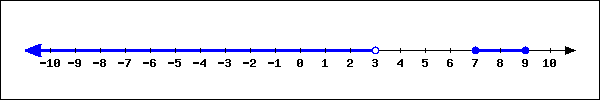
\includegraphics[width=\linewidth]{generated/webwork/images/webwork-17-image-1.png}
\end{image}%
Answer: \fillintext{20}%
\par\smallskip%
\noindent\textbf{\blocktitlefont Answer}.\hypertarget{answer-module-1-s-b}{}\quad{}\(\left(-\infty ,3\right)\cup \left[7,9\right]\)%
\end{inlineexercise}%
\begin{inlineexercise}{Checkpoint}{}{exercise-module-1-t}%
\begin{image}{0.075}{0.85}{0.075}{-1.5\baselineskip}%
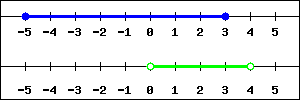
\includegraphics[width=\linewidth]{generated/webwork/images/webwork-18-image-1.png}
\end{image}%
For the graphs shown above, find the following:%
\par
%
\begin{enumerate}[label=\alph*.]
\item{}Write a compound inequality to describe the \emph{union} of the points shown in the graphs.%
\end{enumerate}
%
\par
Answer: \fillintext{5}%
\par
%
\begin{enumerate}[label=\alph*.]
\item{}Write a compound inequality to describe the \emph{intersection} of the points shown in the graphs.%
\end{enumerate}
%
\par
Answer: \fillintext{5}%
\par\smallskip%
\noindent\textbf{\blocktitlefont Answer 1}.\hypertarget{answer-module-1-t-b}{}\quad{}\(\left[-5,4\right)\)%
\par\smallskip%
\noindent\textbf{\blocktitlefont Answer 2}.\hypertarget{answer-module-1-t-c}{}\quad{}\(\left(0,3\right]\)%
\end{inlineexercise}%
\begin{inlineexercise}{Checkpoint}{}{exercise-module-1-u}%
\begin{image}{0.25}{0.5}{0.25}{-1.5\baselineskip}%
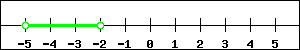
\includegraphics[width=\linewidth]{generated/webwork/images/webwork-19-image-1.png}
\end{image}%
Express the inequality shown in the graph above using interval notation.%
\par
Answer: \fillintext{25}%
\par\smallskip%
\noindent\textbf{\blocktitlefont Answer}.\hypertarget{answer-module-1-u-b}{}\quad{}\(\left(-5,-2\right)\)%
\end{inlineexercise}%
\begin{inlineexercise}{Checkpoint}{}{exercise-module-1-v}%
Write the interval notation for the given graph:%
\par
If the set includes more than one interval, they are joined using the union symbol U.  We use the captial letter of ``u'' as the union symbol.%
\begin{image}{0.075}{0.85}{0.075}{}%
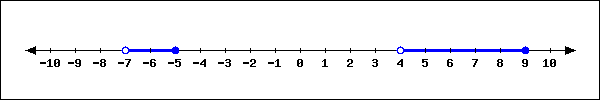
\includegraphics[width=\linewidth]{generated/webwork/images/webwork-20-image-1.png}
\end{image}%
Answer: \fillintext{5}%
\par\smallskip%
\noindent\textbf{\blocktitlefont Answer}.\hypertarget{answer-module-1-v-b}{}\quad{}\(\left(-7,-5\right]\cup \left(4,9\right]\)%
\end{inlineexercise}%
\end{sectionptx}
\end{chapterptx}
%
\backmatter%
%
\clearpage\phantomsection%
\addcontentsline{toc}{part}{Back Matter}%
%
%% The index is here, setup is all in preamble
%% Index locators are cross-references, so same font here
{\xreffont\printindex}
%
\end{document}
